\documentclass[11pt,a4paper]{report}

% Encoding & Language 
\usepackage[utf8]{inputenc}
\usepackage[T1]{fontenc}
\usepackage[french]{babel}

% Fonts 
\usepackage[scaled=0.90]{helvet}
\renewcommand{\familydefault}{\sfdefault}

% Page layout 
\usepackage{geometry}
\geometry{
  a4paper,
  left=25mm,
  right=25mm,
  top=20mm,
  bottom=20mm,
}
\usepackage{titlesec}
\titleformat{\chapter}{}{}{0em}{\bfseries\LARGE}
\usepackage{setspace}
\interlinepenalty=1000
\clubpenalty=10000
\widowpenalty=10000
\displaywidowpenalty=10000

% Colors & Graphics 
\usepackage[table,dvipsnames]{xcolor}
\definecolor{mygreen}{RGB}{198,239,206}
\definecolor{myyellow}{RGB}{255,255,204}
\definecolor{myorange}{RGB}{255,204,153}
\definecolor{myred}{RGB}{255,102,102}
\definecolor{mydarkred}{RGB}{204,0,0}
\definecolor{mydeepred}{RGB}{150,0,0}

\usepackage[normalem]{ulem}
\usepackage{graphicx}
\usepackage{float}
\usepackage{booktabs}
\usepackage{multirow}

% Graphics and Plots
\usepackage{tikz}
\usetikzlibrary{calc, positioning, arrows.meta, shapes.geometric, decorations.pathreplacing}
\usepackage{pgfplots}
\pgfplotsset{compat=1.18}
\usepgfplotslibrary{fillbetween}
\usepackage{pgfplotstable}

% Listings for source code 
\usepackage{listings}
\usepackage{fvextra}

\usepackage[colorlinks=true, linkcolor=blue, urlcolor=teal]{hyperref}

%  Glossaries & Bibliography 
\usepackage[acronym]{glossaries}
\makeglossaries
\newacronym{cristal}{CRIStAL}{Centre de Recherche en Informatique, Signal et Automatique de Lille}
\newacronym{chu}{CHU de Lille}{Centre Hospitalier Universitaire de Lille}
\newacronym{itd}{ITD}{duplication interne en tandem}
\newacronym{mrd}{MRD}{maladie résiduelle détectable}
\newacronym{vdj}{V(D)J}{Variable, Diversité et Jonction}
\newacronym[longplural=immunoglobulines]{ig}{Ig}{immunoglobuline}
\newacronym{igh}{IgH}{chaîne lourde des immunoglobulines}
\newacronym{igk}{Igk}{chaîne légère kappa (\texorpdfstring{$\kappa$}{kappa})}
\newacronym{igl}{Igl}{chaîne légère lambda (\texorpdfstring{$\lambda$}{lambda})}
\newacronym[longplural=récepteurs des cellules T]{tcr}{TCR}{récepteur des cellules T}
\newacronym{tra}{TRA}{récepteur des cellules T alpha (\texorpdfstring{$\alpha$}{alpha})}
\newacronym{trb}{TRB}{récepteur des cellules T bêta (\texorpdfstring{$\beta$}{beta})}
\newacronym{trg}{TRG}{récepteur des cellules T gamma (\texorpdfstring{$\gamma$}{gamma})}
\newacronym{trd}{TRD}{récepteur des cellules T delta (\texorpdfstring{$\delta$}{delta})}
\newacronym{hpc}{HPC}{cluster de calcul haute performance}
\newacronym[longplural=régions \textit{framework}]{fr}{FR}{région \textit{framework} }
\newacronym[
  longplural=régions hypervariables (\textit{complementarity-determining regions})
]{cdr}{CDR}{région hypervariable (\textit{complementarity-determining region})}
 

\usepackage[backend=biber, style=numeric, sorting=none]{biblatex}
\addbibresource{references.bib}

% Captions 
\usepackage{caption}
\captionsetup{
    labelfont={color=gray},
    textfont={color=gray}
}

% Other useful packages 
\usepackage{fontawesome5}
\usepackage{rotating}
\usepackage{amssymb}

% tcolorbox setup 
\usepackage[most]{tcolorbox}
\tcbset{colback=blue!5, colframe=blue!70, boxrule=0.5pt, arc=4pt,
       left=6pt, right=6pt, top=6pt, bottom=6pt}
\newtcolorbox[auto counter, number within=section]{examplebox}[1][]{%
  title=Example~\thetcbcounter, #1
}

% Algorithm2e setup 
\usepackage[french,linesnumbered,ruled,vlined]{algorithm2e}
\SetKwInput{KwIn}{Entrée}
\SetKwInput{KwOut}{Sortie}
\SetKwData{KwData}{Donnée}
\SetKwIF{If}{ElseIf}{Else}{si}{alors}{sinon si}{sinon}{fin si}
\SetKwFor{For}{pour}{faire}{fin}

% Custom commands for nucleotide coloring 
\newcommand{\A}{\textcolor{Cyan}{A}}
\newcommand{\T}{\textcolor{ForestGreen}{T}}
\newcommand{\Tb}{\textcolor{OliveGreen}{\uline{T}}}
\newcommand{\G}{\textcolor{Magenta}{G}}
\newcommand{\C}{\textcolor{Orange}{C}}
\newcommand{\Hbase}{H}
\newcommand{\N}{N}
\newcommand{\Y}{Y}

% Verbatim environment with colors 
\DefineVerbatimEnvironment{ColoredVerbatim}{Verbatim}{
    fontsize=\small,
    commandchars=\\\{\},
    formatcom=\ttfamily
}

% Annex environment 
\usepackage{newfloat}
\DeclareFloatingEnvironment[
    fileext=loa,
    listname=Liste des annexes,
    name=Annexe
]{annex}

% Listings language definitions 
\lstdefinelanguage{json}{
    basicstyle=\normalfont\ttfamily,
    numbers=left,
    numberstyle=\scriptsize,
    stepnumber=1,
    numbersep=8pt,
    showstringspaces=false,
    breaklines=true,
    frame=lines,
    backgroundcolor=\color{blue!5},
    literate=
     *{0}{{{\color{magenta!60!black}0}}}{1}
      {1}{{{\color{magenta!60!black}1}}}{1}
      {2}{{{\color{magenta!60!black}2}}}{1}
      {3}{{{\color{magenta!60!black}3}}}{1}
      {4}{{{\color{magenta!60!black}4}}}{1}
      {5}{{{\color{magenta!60!black}5}}}{1}
      {6}{{{\color{magenta!60!black}6}}}{1}
      {7}{{{\color{magenta!60!black}7}}}{1}
      {8}{{{\color{magenta!60!black}8}}}{1}
      {9}{{{\color{magenta!60!black}9}}}{1}
      {:}{{{\color{red!60!black}{:}}}}{1}
      {,}{{{\color{red!60!black}{,}}}}{1}
      {\{}{{{\color{blue!60!black}{\{}}}}{1}
      {\}}{{{\color{blue!60!black}{\}}}}}{1}
      {[}{{{\color{blue!60!black}{[}}}}{1}
      {]}{{{\color{blue!60!black}{]}}}}{1},
}

\lstdefinelanguage{custombash}{
    sensitive=true,
    morekeywords={
        echo, tr, rev, grep, xargs, cat, cd, ls, mv, cp, rm, touch, mkdir, pwd, head, tail, awk, 
        sed, cut, sort, uniq, find, chmod, chown, bash, sh, if, then, else, fi, for, while, in, do, done,
        CGTCTCCTCAGGTAAG
    },
    otherkeywords={|, >, <, >>, <<, &, &&, ;, !, =, ~, *, \$},
    morecomment=[l]{\#},
    morestring=[b]",
    morestring=[b]',
    showstringspaces=false,
    basicstyle=\ttfamily\small,
    keywordstyle=\color{blue},
    commentstyle=\color{gray},
    stringstyle=\color{red!70!black},
    numberstyle=\tiny\color{gray},
    numbers=left,
    stepnumber=1,
    numbersep=8pt,
    backgroundcolor=\color{blue!5},
    breaklines=true,
    frame=lines,
    literate=
     *{0}{{{\color{magenta!60!black}0}}}{1}
      {1}{{{\color{magenta!60!black}1}}}{1}
      {2}{{{\color{magenta!60!black}2}}}{1}
      {3}{{{\color{magenta!60!black}3}}}{1}
      {4}{{{\color{magenta!60!black}4}}}{1}
      {5}{{{\color{magenta!60!black}5}}}{1}
      {6}{{{\color{magenta!60!black}6}}}{1}
      {7}{{{\color{magenta!60!black}7}}}{1}
      {8}{{{\color{magenta!60!black}8}}}{1}
      {9}{{{\color{magenta!60!black}9}}}{1},
}

\renewcommand{\lstlistingname}{Code}

%  Document start 
\begin{document}

\onehalfspacing

\begin{titlepage}
    \centering
    \vspace*{1cm}

    {\Large \textbf{Université de Lille}}\\[0.5cm]
    {\large Faculté des Sciences et Technologies}\\[0.5cm]
    {\large Master 2 Méthodes Informatiques et Statistiques pour les OMICS}\\[2cm]

    {\Huge \bfseries Developpements bioinformatiques appliqués à l'étude du myélome multiple}\\[1cm]
    {\LARGE \textit{Approche pour l'étude de la maladie résiduelle par recombinaisons V(D)J sur la plateforme Vidjil}}\\[2.5cm]

    \begin{flushleft}
    \textbf{Présenté par :} Ilyès Benhalima\\
    \textbf{Encadrants :}
    \begin{tabular}[t]{@{}l}
        Mikaël Salson (Professeur des universités, FST) \\
        Augustin Boudry (Assistant Hospitalo-Universitaire, CHU de Lille)
    \end{tabular}\\

    \vspace{1em}

    \textbf{Tuteur universitaire :} Guillaume Brysbaert (Ingénieur de recherche, CNRS)\\[1.5cm]

    \textbf{Année universitaire :} 2024-2025\\
    \textbf{Date de soutenance :} 5 septembre 2025\\
    \end{flushleft}

    \vfill

    \textit{Mémoire présenté en vue de l'obtention du diplôme de Master 2}\\[2cm]

    \begin{minipage}{0.30\textwidth}
        \centering
        
\includegraphics[width=1\textwidth]{images/logo_fst_ulille_cropped.png}
    \end{minipage}
    \hfill
    \begin{minipage}{0.30\textwidth}
        \centering
        
\includegraphics[width=0.8\textwidth]{images/logo_cristal.png}
    \end{minipage}
    \hfill
    \begin{minipage}{0.30\textwidth}
        \centering
        
\includegraphics[width=0.8\textwidth]{images/logo_chu.jpg}
    \end{minipage}

\end{titlepage}

\chapter*{Remerciements}

Merci.

\tableofcontents

\printglossaries

\chapter{Préambule}

Ce stage a été réalisé conjointement entre l'équipe Bonsai du \gls{cristal}, 
dirigée par le Pr. Mikaël Salson, également encadrant de ce travail, 
et l'équipe de bioinformatique du \gls{chu}, coordonnée par Martin Figeac. 
Il s'inscrit dans une collaboration de longue date entre ces deux équipes, 
et notamment en interaction étroite avec le laboratoire d'Hématologie du Pr. Claude Preudhomme, 
qui bénéficie de l'expertise du laboratoire Bonsai dans le domaine de la bioinformatique 
des séquences.

\vspace{1em}

L'équipe Bonsai, au sein du laboratoire \gls{cristal}, regroupe des chercheurs et enseignants-chercheurs
spécialisés en bioinformatique, algorithmique et modélisation des données biologiques. 
Elle développe notamment des méthodes innovantes pour l'analyse des séquences génomiques, 
via des approches d'algorithmique du texte et structures d'index, avec un accent particulier 
sur les méthodes sans alignements. 

\vspace{1em}

L'équipe de bioinformatique du \gls{chu}, quand à elle, 
s'inscrit dans une dynamique translationnelle forte entre recherche et application clinique. 
Elle travaille en étroite collaboration avec les thématiques médicales, notamment en onco-hématologie, 
pour concevoir et appliquer des outils bioinformatiques performants dans le suivi et le diagnostic des patients.
Elle regroupe 12 ingénieurs et techniciens concourant au développement et maintien de solutions bioinformatiques,
pour l'analyse de données de \gls{ngs}, mais aussi la gestion d'un parc informatique riche doté 
d'un \gls{hpc} et la conception d'outils et solutions utilisateurs et développeurs.

\vspace{1em}

Cette collaboration a donné naissance à plusieurs projets et outils 
largement diffusés et utilisés dans la communauté scientifique, 
et plus particulièrement dans le domaine médical, où ils font aujourd'hui figure de référence. 
Parmi ceux-ci, on peut citer l'outil \textit{FiLT3r}, permettant la détection 
et la quantification des variants de type \gls{itd} du gène \textit{FLT3} \cite{boudryFrugalAlignmentfreeIdentification2022}, 
ainsi que la plateforme \textit{Vidjil} \cite{duezVidjilWebPlatform2016}, dédiée à l'étude des répertoires immunitaires B et T.

\vspace{1em}

C'est concernant ce dernier outil que s'inscrit ce stage, dans la continuité de travaux précédents,
avec l'objectif d'adapter et de développer de nouvelles fonctionnalités via \textit{Vidjil} 
pour l'analyse de la \gls{mrd} dans les hémopathies malignes lymphoïdes, en particulier dans le myélome multiple.
\chapter{Introduction}

\textit{Vidjil} est une plateforme open-source
\cite{giraudFastMulticlonalClusterization2014b} permettant l'analyse de données
de \gls{ngs} pour l'étude du répertoire des gènes \gls{vdj} des cellules
lymphoïdes. Ce processus de recombinaison somatique se produit au sein des
précurseurs B et T lors de la lymphopoïèse, et permet de générer un vaste
répertoire d'anticorps et de récepteurs, capables à leur tour de reconnaître une
grande variété d'antigènes \cite{jonesTamingTransposonVDJ2004}. \textit{Vidjil}
trouve ses applications en immunologie pour l'étude de la diversité du
répertoire immunitaire ainsi qu'en hématologie, où il permet une analyse fine
des répertoires V(D)J dans les hémopathies lymphoïdes pour en affiner le
diagnostic et le suivi.

\section{Répertoire et recombinaison des gènes V(D)J}

% Alors ici ta section est top ! très bien écrite et très claire. Cependant
% Chaîne lourde etc. pop de nul part je trouve. Pas sûr que la personne qui lise
% ton mémoire soit au courant. j'ai juste modifié l'ordre ;) ca me parait plus
% clair. et j'ai retiré ce qui concerne les TCRs ça te permet de garder en
% clarté je pense.

Ce processus de recombinaison est complexe, et implique plusieurs étapes successives de réarrangement des segments \gls{vdj} 
au sein des loci des \glspl{ig} et des \glspl{tcr} \cite{rothVDJRecombinationMechanism2014}. Les \glspl{ig} sont des récepteurs membranaires 
ou des anticorps solubles exprimés par les lymphocytes B, tandis que les \glspl{tcr} sont exprimés à la surface des lymphocytes T et permettent 
la reconnaissance des antigènes présentés par le \gls{cmh}.

\vspace{1em}

Dans le cadre de ce travail, seules les recombinaisons des \glspl{ig}, et plus
précisément de la chaîne lourde \textit{\gls{igh}}, seront prises en compte,
pour des raisons qui apparaîtront rapidement évidentes\footnote{La pathologie
étudiée étant d'origine lymphocytaire B, seuls les réarrangements impliqués dans
la production des anticorps, c'est-à-dire les réarrangements \textit{IgH}, et
dans une moindre mesure \textit{IgK} et \textit{IgL} sont pertinents.}.

\vspace{1em}

La recombinaison débute par la sélection aléatoire de segments D et J, suivie de la sélection d'un segment V, au sein des chaînes dites « lourdes », 
sous l'action des recombinases \gls{vdj}. Un mécanisme identique est observé pour les chaînes « légères », avec une recombinaison directe des segments V et J, 
sans étape D. À la suite de chaque recombinaison, des régions de diversité N de quelques nucléotides sont insérées aléatoirement entre les segments, 
contribuant à la diversité potentielle du répertoire (\autoref{fig:vdj}). Par conséquent, si l'on considère les loci des \glspl{ig}, la recombinaison \gls{vdj} 
permet de générer théoriquement : 

\begin{examplebox}[label={ex:combinaisons}]
    \begin{equation}
        \begin{aligned}
        \text{Chaîne lourde : } & \underbrace{50}_{\text{\# VH}} \times \underbrace{30}_{\text{\# DH}} \times \underbrace{6}_{\text{\# JH}} = 9000 \\
        \text{Chaîne légère } \kappa : & \underbrace{40}_{\text{\# Vk}} \times \underbrace{5}_{\text{\# Jk}} = 200 \\
        \text{Chaîne légère } \lambda : & \underbrace{46}_{\text{\# Vl}} \times \underbrace{7}_{\text{\# Jl}} = 322 \\
        \text{Total des combinaisons possibles : } & 9000 \times (200 + 322) = 4\,698\,000
        \end{aligned}
    \end{equation}
\end{examplebox}

Soit près de 5 millions de combinaisons possibles, en sachant que l'ajout des régions de diversité N
et des différentes régions constantes porte ce nombre à une valeur presque infinie (example \autoref{ex:combinaisons}).

\vspace{1em}

Ainsi, \textit{Vidjil} permet l'analyse des réarrangements des \glspl{ig} présents sur les loci suivants : 
\begin{itemize}
    \item \textit{\gls{igh}} sur le chromosome 14, 
    \item \textit{\gls{igk}} sur le chromosome 2, 
    \item \textit{\gls{igl}} sur le chromosome 22.
\end{itemize}

\begin{figure}[H]
    \centering
    \begin{tikzpicture}[
        node distance=0.3cm and 0cm,
        >=Stealth,
        thick,
        font=\small,
        scale=0.95,
        every node/.style={scale=0.95}
        ]

    % Chaîne lourde : segments germinaux 
    \foreach \name/\label/\i in {v1/V1/0, v2/V2/1, v3/V3/2, v4/V\dots/3, vn/Vn/4} {
        \node[rectangle, draw, fill=blue!20, minimum width=1.3cm, minimum height=0.8cm]
            (\name) at ($(0,0)+(1.4*\i,0)$) {\label};
    }

    \foreach \name/\label/\i in {d1/D1/0, d2/D\dots/1, dn/DN/2} {
        \node[rectangle, draw, fill=green!30, minimum width=0.4cm, minimum height=0.8cm]
            (\name) at ($(vn.east)+(1.1+0.8*\i,0)$) {\label};
    }

    \foreach \name/\label/\i in {j1/J1/0, j2/J2/1, j3/J\dots/2, jn/JN/3} {
        \node[rectangle, draw, fill=orange!30, minimum width=0.6cm, minimum height=0.8cm]
            (\name) at ($(dn.east)+(1.1+0.8*\i,0)$) {\label};
    }

    \node[rectangle, draw, right=0.5cm of jn, fill=gray!30, minimum width=2cm, minimum height=0.8cm] (c) {C};

    \draw[thick] ($(vn.east)+(0,-0.1)$) -- ($(d1.west)+(0,-0.1)$);
    \draw[thick] ($(dn.east)+(0,-0.1)$) -- ($(j1.west)+(0,-0.1)$);
    \draw[thick] ($(jn.east)+(0,-0.1)$) -- ($(c.west)+(0,-0.1)$);

    \node[anchor=west] at ($(v1.north west)+(0,0.4cm)$) {\textbf{Segments germinaux - chaîne lourde}};

    \node at ($(v1.west)+(-0.3,0)$) {\textbf{5'}};
    \node at ($(c.east)+(0.3,0)$) {\textbf{3'}};

    % Recombinaison D-J 
    \node[rectangle, draw, below=2cm of c, fill=gray!30, minimum width=2cm, minimum height=0.8cm] (c_bis) {C};
    \node[rectangle, draw, left=0.5cm of c_bis, fill=orange!30, minimum width=0.6cm, minimum height=0.8cm] (j_recomb) {J};
    \node[rectangle, draw, left=of j_recomb, fill=red!20, dashed, minimum width=0.3cm, minimum height=0.8cm] (n1) {N};
    \node[rectangle, draw, left=of n1, fill=green!30, minimum width=0.4cm, minimum height=0.8cm] (d_recomb) {D};

    \foreach \name/\label/\i in {v1_bis/V1/0, v2_bis/V2/1, v3_bis/V3/2, v4_bis/V\dots/3, vn_bis/Vn/4} {
        \node[rectangle, draw, fill=blue!20, minimum width=1.3cm, minimum height=0.8cm]
            (\name) at ($(d_recomb.east)+(-7.5+1.4*\i,0)$) {\label};
    }

    \draw[thick] ($(vn_bis.east)+(0,-0.1)$) -- ($(d_recomb.west)+(0,-0.1)$);
    \draw[thick] ($(j_recomb.east)+(0,-0.1)$) -- ($(c_bis.west)+(0,-0.1)$);

    \draw[->, thick] (d2.south) -- (d_recomb.north);
    \draw[->, thick] (j2.south) -- (j_recomb.north);

    \node[anchor=west] at ($(v1_bis.north west)+(0,0.4cm)$) {\textbf{Recombinaison D-J}};

    % Recombinaison V-DJ 
    \node[rectangle, draw, below=2cm of c_bis, fill=gray!30, minimum width=2cm, minimum height=0.8cm] (c_bis2) {C};
    \node[rectangle, draw, left=of c_bis2, fill=orange!30, minimum width=0.6cm, minimum height=0.8cm] (j_final) {J};
    \node[rectangle, draw, left=of j_final, fill=red!20, dashed, minimum width=0.3cm, minimum height=0.8cm] (n2) {N};
    \node[rectangle, draw, left=of n2, fill=green!30, minimum width=0.4cm, minimum height=0.8cm] (d_final) {D};
    \node[rectangle, draw, left=of d_final, fill=red!20, dashed, minimum width=0.3cm, minimum height=0.8cm] (n3) {N};
    \node[rectangle, draw, left=of n3, fill=blue!20, minimum width=1.3cm, minimum height=0.8cm] (v_final) {V};

    \draw[thick] ($(j_final.east)+(0,-0.1)$) -- ($(c_bis2.west)+(0,-0.1)$);
    \draw[->, thick] (v2_bis.south) -- (v_final.north);

    \node[anchor=west] at ($(v_final.north west)+(0,0.4cm)$) {\textbf{Recombinaison V-(D)J}};

    %  Chaîne légère : segments germinaux 
    \foreach \name/\label/\i in {vl1/V1/0, vl2/V2/1, vl3/V3/2, vl4/V\dots/3, vln/Vn/4} {
        \node[rectangle, draw, fill=blue!5, rotate=90, minimum width=1.3cm, minimum height=0.8cm]
            (\name) at ($(0,-2.5)+(0,-1.4*\i)$) {\label};
    }

    \foreach \name/\label/\i in {jl1/J1/0, jl2/J2/1, jl3/J\dots/2, jln/JN/3} {
        \node[rectangle, draw, fill=orange!5, rotate=90, minimum width=0.6cm, minimum height=0.8cm]
            (\name) at ($(vln.east)+(0,-2)+(0,-0.8*\i)$) {\label};
    }

    \draw[thick] ($(vln.west)+(0,0)$) -- ($(jl1.east)+(0,0)$);

    \node[rectangle, draw, rotate=90, left=of jln, fill=gray!5, minimum width=3cm, minimum height=0.8cm] (cl) {C};
    \node[anchor=east, rotate=90] at ($(jl1.north west)+(-0.4,3cm)$) {\textbf{Segments germinaux - chaîne légère}};

    \node[rotate=90] at ($(vl1.east)+(0,0.3)$) {\textbf{5'}};
    \node[rotate=90] at ($(cl.west)+(0,-0.3)$) {\textbf{3'}};

    % Recombinaison V-J (chaine légère) 
    \node[rectangle, draw, right=3cm of cl, rotate=90, fill=gray!5, minimum width=3cm, minimum height=0.8cm] (cl_bis) {C};
    \node[rectangle, draw, right=of cl_bis, rotate=90, fill=orange!5, minimum width=0.6cm, minimum height=0.8cm] (jl_final) {J};
    \node[rectangle, draw, right=of jl_final, rotate=90, fill=red!5, dashed, minimum width=0.3cm, minimum height=0.8cm] (nl) {N};
    \node[rectangle, draw, right=of nl, rotate=90, fill=blue!5, minimum width=1.3cm, minimum height=0.8cm] (vl_final) {V};

    \draw[->, thick] (vl3.south) -- (vl_final.north);
    \draw[->, thick] (jl1.south) -- (jl_final.north);

    \node[anchor=west, rotate=90] at ($(cl_bis.north west)+(-0.4,0cm)$) {\textbf{Recombinaison V-J}};

    % Assemblage final : fragment d'immunoglobuline 
    \node[draw, fill=orange!30, rounded corners=8pt, rotate=45, minimum width=0.3cm, minimum height=1cm] at (7.5,-8) (j_ig) {J};
    \node[draw, fill=green!30, rounded corners=8pt, rotate=45, minimum width=0.3cm, minimum height=1cm, right=of j_ig] (d_ig) {D};
    \node[draw, fill=blue!20, rounded corners=8pt, rotate=45, minimum width=0.3cm, minimum height=1cm, right=of d_ig] (v_small_ig) {V};
    \node[draw, fill=blue!20, rounded corners=8pt, rotate=-45, minimum width=1.5cm, minimum height=1.3cm] at (8.8,-8.6) (v_ig) {VH};
    \node[draw, fill=gray!20, rounded corners=8pt, rotate=-45, minimum width=2cm, minimum height=1.3cm, right=of v_ig] (ch1) {CH1};
    \node[draw, fill=gray!20, rounded corners=8pt, rotate=-90, minimum width=2cm, minimum height=1.3cm] at (11,-12) (ch2) {CH2};
    \node[draw, fill=gray!20, rounded corners=8pt, rotate=-90, minimum width=2cm, minimum height=1.3cm, right=of ch2] (ch3) {CH3};
    \node[draw, fill=gray!5, below=0cm of ch1, rounded corners=8pt, rotate=-45, minimum width=2cm, minimum height=0.7cm] (clf) {CL};
    \node[draw, fill=blue!5, left=of clf, rounded corners=8pt, rotate=-45, minimum width=2.6cm, minimum height=0.7cm] (vj) {VL-JL};

    \draw[->, thick] (v_final.south) -- (v_small_ig.north);
    \draw[->, thick] (d_final.south) -- (d_ig.north);
    \draw[->, thick] (j_final.south) -- (j_ig.north);
    \draw[->, thick] (vl_final.south) -- (vj.west);
    \draw[->, thick] (jl_final.south) -- (vj.west);

    \end{tikzpicture}
    \caption{
        Étapes successives de la recombinaison \gls{vdj} des loci des immunoglobulines. 
        \colorbox{blue!20}{V}, \colorbox{green!30}{D}, \colorbox{orange!30}{J} : segments \textbf{Variables}, \textbf{Diversité} et \textbf{Jonction} ; 
        \colorbox{gray!30}{C} : régions \textbf{Constante} ; 
        \colorbox{red!20}{N} : régions de \textbf{N-diversité} ; 
        \textbf{H} : parties lourdes (\textbf{Heavy}) ; 
        \textbf{L} : parties légères (\textbf{Light}). 
        En haut : chaîne lourde ; à gauche : chaîne légère ; 
        en bas : schéma d'un fragment d'immunoglobuline complète.
    }    
    \label{fig:vdj}
\end{figure}


\vspace{1em}

Si l'on s'intéresse plus en détail à la structure des remaniements \gls{vdj} des \textit{\gls{igh}},
on peut noter que les segments codant la région variable de la chaîne lourde (V, D et J)
incluent plusieurs sous-régions fonctionnelles. En amont du segment V, on trouve la région \textit{leader} et 
le segment V lui-même est divisé en \glspl{fr} 1, 2 et 3, qui assurent le repliement structural du domaine variable 
\footnote{Et servent de matrice pour la conception d'amorces d'amplification par \gls{pcr}.}, 
et les \glspl{cdr} (\autoref{fig:igh}). Parmi celles-ci, la région \gls{cdr}3, située à la jonction des segments V, D et J 
est la plus variable et joue un rôle central dans la reconnaissance de l'antigène, et l'unicité du réarrangement.

\vspace{1em}

La diversité de cette région \gls{cdr}3 est générée par plusieurs mécanismes :
la recombinaison somatique entre les segments V, D et J, et l'ajout des domaines de N-diversité 
mentionnés précédemment, mais aussi l'excision de nucléotides en 3' et 5' des segments V, D et J.
À cela s'ajoute un processus d'hypermutation somatique, qui affecte principalement le segment V 
après activation des lymphocytes B naïf, introduisant des mutations ponctuelles supplémentaires,
notamment dans les régions \glspl{cdr}, afin d'augmenter l'affinité de l'anticorps pour son antigène (\autoref{fig:igh}).

\begin{figure}[H]
    \centering
    \begin{tikzpicture}[node distance=0cm, thick, font=\tiny]

    % Segments avec séquences nucléotidiques
    \node[rectangle, fill=blue!20, minimum width=6cm, minimum height=0.8cm, anchor=west] (v_full) at (0,0)
        {\shortstack{\textbf{VH3-30} \\ \dots ATGAATAGCCTGAGGCCT\textcolor{red}{G}AGGACACGGCTG\textcolor{red}{TG}TATTAC\textcolor{red}{T}GTAC\sout{A}}};

    \node[rectangle, right=of v_full, fill=red!20, dashed, minimum width=0.6cm, minimum height=0.8cm] (n1_full)
        {\shortstack{\textbf{N} \\ AAAGGGGTGGAC}};

    \node[rectangle, right=of n1_full, fill=green!20, minimum width=1.5cm, minimum height=0.8cm] (d_full)
        {\shortstack{\textbf{D3-3} \\ \sout{CG}ATGTTTGGAGT\sout{GGTT}}};

    \node[rectangle, right=of d_full, fill=red!20, dashed, minimum width=0.6cm, minimum height=0.8cm] (n2_full)
        {\shortstack{\textbf{N} \\ TCG}};

    \node[rectangle, right=of n2_full, fill=orange!20, minimum width=2cm, minimum height=0.8cm] (j_full)
        {\shortstack{\textbf{J4*02} \\ \sout{ACTGGGGCCAGG}GAACCCT\dots}};

    % Régions 3' et 5'
    \node[left=0.2cm of v_full.west] {\scriptsize \textbf{5'}};
    \node[right=0.2cm of j_full.east] {\scriptsize \textbf{3'}};

    % Régions fonctionnelles
    \draw[thick, blue] ($(v_full.west)+(-1,-0.6)$) -- ++(1,0) node[midway, below=2pt] {\scriptsize Leader};
    \draw[thick, blue] ($(v_full.west)+(0.7,-0.6)$) -- ++(1,0) node[midway, below=2pt] {\scriptsize FR1};
    \draw[thick, blue] ($(v_full.west)+(2,-0.6)$) -- ++(1,0) node[midway, below=2pt] {\scriptsize FR2};
    \draw[thick, blue] ($(v_full.west)+(4.7,-0.6)$) -- ++(1,0) node[midway, below=2pt] {\scriptsize FR3};

    \draw[thick, red] ($(v_full.east)+(-0.5,+0.6)$) -- ($(j_full.west)+(0.5,+0.6)$)
        node[midway, above=1.5pt] {\scriptsize \textbf{CDR3}};

    % Nom du réarrangement
    \node[below=1.5cm of n1_full.center, anchor=center, font=\large] {
        \textcolor{blue!60!black}{\texttt{IGHV3-30 1}}\,/%
        \textcolor{red!70!black}{\texttt{AAAGGGGTGGAC(12)}}\,/%
        \textcolor{green!70!black}{\texttt{2}}\,%
        \textcolor{green!70!black}{\texttt{D3-3 4}}\,/%
        \textcolor{red!70!black}{\texttt{TCG}}\,/%
        \textcolor{orange!80!black}{\texttt{12}}
        \textcolor{orange!80!black}{\texttt{J4*02}}
    };
    
    \end{tikzpicture}
    \caption{Illustration d'un réarrangement de la chaîne lourde des immunoglobulines \gls{igh}.
    Les bases rayées correspondent aux nucélotides excisés lors de la recombinaison. 
    Les \textcolor{red}{bases en rouge} sont celles mutées par rapport aux séquences germinales lors du 
    processus d'hypermutation somatique.}
    \label{fig:igh}
\end{figure}


Chaque réarrangement \gls{vdj} peut être décrit à l'aide d'une nomenclature standardisée, 
permettant une identification unique et reproductible \cite{laneIMGTONTOLOGYIMGTLIGMotif2010,lefrancIMGT30Years2019}. 
Cette notation précise la nature du locus considéré, le segment V utilisé, les nucléotides excisés à son extrémité 3', 
la séquence ou longueur de la première région N insérée, le segment D (le cas présent) avec ses excisions en 3' et 5' 
et la seconde région N, ainsi que le segment J retenu et son excision en 5' (\autoref{tab:nomenclature-vdj}).

\begin{table}[H]
    \centering
    \caption{Nomenclature d'un réarrangement \gls{vdj}, BE : Bases excisées.}
    \label{tab:nomenclature-vdj}
    \begin{tabular}{c c c c c c c c c c}
        \toprule
        \textbf{Locus} & \textbf{VH} & \textbf{BE V3'} & \textbf{N1} & \textbf{BE D5'} & 
        \textbf{D Nom} & \textbf{BE D3'} & \textbf{N2} & \textbf{BE J5'} & \textbf{J Nom} \\        
        \midrule IGH & VH3-30 & 1 & 12 & 2 & D3-3 & 4 & TCG & 12 & J4*02 \\
        \bottomrule
    \end{tabular}
\end{table}


\section{Détection et visualisation des réarrangements V(D)J via \textit{Vidjil}}

La plateforme \textit{Vidjil} qui permet donc l'étude de ces réarrangements \gls{vdj} est développée et maintenue 
conjointement par l'équipe Bonsai du laboratoire \gls{cristal} et par le consortium \textit{VidjilNet}. 
Elle regroupe d'une part l'algorithme \textit{vidjil-algo}, une heuristique de détection des réarrangement \gls{vdj} 
\cite{giraudFastMulticlonalClusterization2014b} et d'autre part une interface web permettant de visualiser les 
résultats ainsi produits \cite{duezVidjilWebPlatform2016}. L'ensemble du code source est disponible sur le dépôt gitlab 
public suivant : \href{https://gitlab.inria.fr/vidjil/vidjil}{gitlab.inria.fr/vidjil/vidjil}.

\vspace{1em}

La première composante, \textit{vidjil-algo} est un programme écrit en \texttt{C++}, dont la fonction est d'extraire 
les jonctions \gls{vdj} à partir des \textit{reads} (lectures) issues du \gls{ngs} dans des fichiers de séquences 
brutes au format FASTQ, ou bien préalablement alignées au format \gls{bam}. Pour ce faire, l'algorithme 
repose sur une heuristique originale qui détecte des fenêtres caractéristiques chevauchant les régions CDR3, 
sans recourir à un alignement exhaustif contre les séquences germinales. Une première étape consiste à constuire un index 
des séquences germinales V et J à partir de \textit{k-mers} (ou mots de taille $\mathbf{k}$), où $\mathbf{k}$ est choisi de façon à 
minimiser les \textit{k-mers} communs aux deux segments (\autoref{fig:index}). L'utilisation de \textit{k-mers} espacés permet d'améliorer la sensibilité 
notamment en cas de substitutions (example \ref{ex:spaced-seed}).

\begin{examplebox}[label={ex:spaced-seed}]
    Le mot \texttt{ATTCG-CAGGT} issue de la graine \texttt{\#\#\#\#\#\#-\#\#\#\#\#} 
    est présent dans la séquence \texttt{ATTCG\textcolor{gray}{G}CAGGT} ou \texttt{ATTCG\textcolor{gray}{T}CAGGT} 
    mais pas \texttt{A\textcolor{red}{C}TCG\textcolor{gray}{A}CAGGT}.
\end{examplebox}

\begin{figure}[H]
    \centering
    \begin{tikzpicture}[node distance=0cm, thick, font=\small]

    % Séquence VH
    \node[anchor=west] (VH) at (0,0) 
    {\shortstack{\textbf{Séquence VH} \\ \textbf{\textcolor{blue}{CATCCGCGAGCACAGCCTACATGG\dots}}}};
    
    % k-mer espacés séquence VH
    \foreach \i [count=\j from 0] in {
        CATCC--CGAGC,
        ATCCG--GAGCA,
        TCCGC--AGCAC,
        CCGCG--GCACA,
        CGCGA--CACAG,
        \dots
    } {
        \pgfmathsetmacro\xshift{\j*0.225}
        \pgfmathsetmacro\ypos{-0.5*(\j+1.1)}
        \node[anchor=west] at (\xshift,\ypos) {\i};
    }

    % Séquence JH
    \node[anchor=west] (J) at (7,0)
    {\shortstack{\textbf{Séquence JH} \\ \textbf{\textcolor{orange}{TGATATCTGGGGCCAAGGGAC\dots}}}};

    % k-mer espacés séquence JH
    \foreach \i [count=\j from 0] in {
        TGATA--CTGGG,
        GATAT--TGGGG,
        ATATC--GGGGC,
        TATCT--GGGCC,
        ATCTG--GGCCA,
        \dots
    } {
        \pgfmathsetmacro\xshift{7 + \j*0.215}
        \pgfmathsetmacro\ypos{-0.5*(\j+1.1)}
        \node[anchor=west] at (\xshift,\ypos) {\i};
    }

    \end{tikzpicture}
    \caption{Génération de l'index à partir de \textit{k-mer} des séquences germinales 
    \textcolor{blue}{VH (à gauche)} et \textcolor{orange}{JH (à droite)}.}
    \label{fig:index}
\end{figure}

    
La seconde étape consiste à traverser l'ensemble des \textit{reads} en recherchant des fenêtres $\mathbf{w}$ qui recouvrent 
la région \gls{cdr}3 par comparaison de chacun des \textit{k-mer} du \textit{read} à ceux des index générés. Brièvement cette 
approche consiste à conserver les \textit{reads} qui contiennent les \textit{k-mer} d'une séquence V et ceux d'une séquence J, 
de façon à former une fenêtre $\mathbf{w}$ débutant par les derniers \textit{k-mer} de la séquence V et se terminant 
par les premiers \textit{k-mer} de la séquence J (\autoref{fig:vidjil-algo}).
Cette approche permet une détection rapide (qui croit linéairement avec le nombre de nucléotides \footnote{En pratique l'étape de détection des fenêtres 
est de compléxité $O(ln)$ et plus récemment $O(l'n)$ où $l$ est le nombre de recombinaisons des systèmes, $l'$ le nombre moyen avec $l' \ll l$, et $n$ 
la taille de la séquence.}), robuste et efficace 
des séquences recombinées. Une fois les fenêtres détectées, \textit{vidjil-algo} regroupe les \textit{reads} en clones, 
puis procède à une segmentation et une annotation des séquences identifiées \footnote{Cette étape de désignation est elle de compléxité $O(Mn)$, et $O(M'n)$ à présent, 
$M$ désignant la taille totale des gènes considérés, et $M'$ un sous ensemble tel que $M' \ll M$.}. 

\begin{figure}[H]
    \centering
    \begin{tikzpicture}[node distance=0cm, thick, font=\small]

    % Première ligne
    \node[
        rectangle, 
        fill=blue!30, 
        text width=4cm, 
        align=left,
        minimum width=4cm, 
        minimum height=0.6cm
        ] at (0,0) (v_predicted1) {VVVVVV};

    \node[right=of v_predicted1] (sub) {\textcolor{red}{X}};

    \node[
        rectangle, 
        right=of sub, 
        fill=blue!30, 
        text width=3cm, 
        align=left,
        minimum width=3cm, 
        minimum height=0.6cm
        ] (v_predicted2) {VVVVVVVVVV};

    \node[
        rectangle, 
        right=2cm of v_predicted2, 
        fill=orange!30, 
        text width=5cm, 
        align=left,
        minimum width=5cm, 
        minimum height=0.6cm
        ] (j_predicted) {JJJJJJJJJJJJJJJJJJ};

    % Fenêtre w
    \draw[draw=violet, thick]
        ($(v_predicted2.west)!0.5!(v_predicted2.east) + (0,0.35)$) rectangle
        ($(j_predicted.west)!0.5!(j_predicted.east) + (0,-0.35)$);

    % Annotations
    \node[anchor=north west] at ([yshift=-1pt]v_predicted1.south west) 
        {\scriptsize \textbf{\textcolor{blue}{V prédit}}};

    \draw[thick, blue] ($(v_predicted1.west)+(0,-0.8)$) -- ($(v_predicted2.east)+(0,-0.8)$) 
        node[anchor=north west] at ([yshift=-0.5cm]v_predicted1.south west) 
        {\scriptsize \textcolor{blue}{V réel}};

    \node[anchor=north east] at ([yshift=-1pt]j_predicted.south east) 
        {\scriptsize \textbf{\textcolor{orange}{J prédit}}};

    \draw[thick, orange] ($(j_predicted.west)+(0,-0.8)$) -- ($(j_predicted.east)+(0,-0.8)$) 
        node[anchor=north east] at ([yshift=-0.5cm]j_predicted.south east) 
        {\scriptsize \textcolor{orange}{J réel}};
        
    \node[above=3pt of sub] {\scriptsize \textbf{\textcolor{red}{Substitution}}};

    \node at ($(v_predicted2)!0.5!(j_predicted)+(0,0.6)$) {\scriptsize \textbf{\textcolor{violet}{Fenêtre extraite w}}};

    % Deuxième ligne
    \begin{scope}[yshift=-2cm]

    \node[
        rectangle, 
        fill=blue!30, 
        text width=4cm, 
        align=left,
        minimum width=4cm, 
        minimum height=0.6cm
        ] at (0,0) (v_predicted1b) {VVVVVVVVVVVV};

    \node[
        rectangle, 
        right=-0.5 cm of v_predicted1b, 
        fill=blue!30,
        minimum width=2.5cm, 
        minimum height=0.6cm
        ] (v_predicted2b) {};

    \node[right=of v_predicted2b] (subb) {\textcolor{red}{X}};

    \node[
        rectangle, 
        right=3.7cm of v_predicted2b, 
        fill=orange!30, 
        text width=5cm, 
        align=left,
        minimum width=5cm, 
        minimum height=0.6cm
        ] (j_predictedb) {JJJJJJJJJJJJJJJJJJ};

    % Fenêtre w
    \draw[draw=violet, thick]
        ($(v_predicted2b.west)!0.5!(v_predicted2b.east) + (0,0.35)$) rectangle
        ($(j_predictedb.west)!0.4!(j_predictedb.east) + (0,-0.35)$);

    % Annotations
    \node[anchor=north west] at ([yshift=-1pt]v_predicted1b.south west) 
        {\scriptsize \textbf{\textcolor{blue}{V prédit}}};

    \draw[thick, blue] ($(v_predicted1b.west)+(0,-0.8)$) -- ($(v_predicted2b.east)+(1.7,-0.8)$) 
        node[anchor=north west] at ([yshift=-0.5cm]v_predicted1b.south west) 
        {\scriptsize \textcolor{blue}{V réel}};

    \node[anchor=north east] at ([yshift=-1pt]j_predictedb.south east) 
        {\scriptsize \textbf{\textcolor{orange}{J prédit}}};

    \draw[thick, orange] ($(j_predictedb.west)+(0,-0.8)$) -- ($(j_predictedb.east)+(0,-0.8)$) 
        node[anchor=north east] at ([yshift=-0.5cm]j_predictedb.south east) 
        {\scriptsize \textcolor{orange}{J réel}};
        
    \node[above=3pt of subb] {\scriptsize \textbf{\textcolor{red}{Substitution}}};

    \node at ($(v_predicted2b)!0.7!(j_predictedb)+(0,0.6)$) {\scriptsize \textbf{\textcolor{violet}{Fenêtre extraite w}}};

    \end{scope}

    \end{tikzpicture}
    \caption{Illustration du fonctionnement de \textit{vidjil-algo} sur deux lectures successives.}
    \label{fig:vidjil-algo}
\end{figure}


Les résultats ainsi générés par \textit{vidjil-algo} sont rassemblés dans un fichier \textit{.vidjil} au format \gls{json} où 
l'on retrouvera des métadonnées en lien avec l'échantillon analysé et un ensemble de données relatif à chaque clone 
identifié par \textit{vidjil-algo} (\autoref{lst:json-vidjil}).

\begin{figure}[H]
\begin{lstlisting}[language=json, 
caption={Extrait d'une sortie de \textit{vidjil-algo}.},
label={lst:json-vidjil}]
"clones": [
    {
        "_average_read_length": ["151.80"],
        "_coverage_info": [ "132 bp (86% of 151.8 bp)"],
        "germline": "IGH",
        "id": "GGGGATAAATTACGATTTTTGGAGTGGTTATTAT...GGGGGTT",
        "name": "IGHV1-8*01 0/CGGGGGGATAA/2 IGHD3-3*01 0/GGTATGGGGGGTTTTAG/7 IGHJ4*02",
        "reads": [498126],
        ...
    }
]
\end{lstlisting}
\end{figure}

En parallèle, \textit{Vidjil} désigne également l'application web \footnote{\url{https://app.vidjil.org/}} 
permettant de visualiser et de manipuler les résultats produits par \textit{vidjil-algo}. 
Elle prend aussi en charge la création et la gestion des comptes utilisateurs, des profils patients, etc. (\autoref{fig:vidjil-web}). 
L'application est développée côté serveur en \texttt{Python}, à l'aide du \textit{framework} \href{https://py4web.com}{\texttt{py4web}} 
(anciennement \texttt{web2py}), et côté client en \texttt{JavaScript}. La base de données utilisée est \texttt{MySQL}, 
le tout étant orchestré via le déploiement de conteneurs \texttt{Docker}.

\begin{figure}[H]
    \centering
    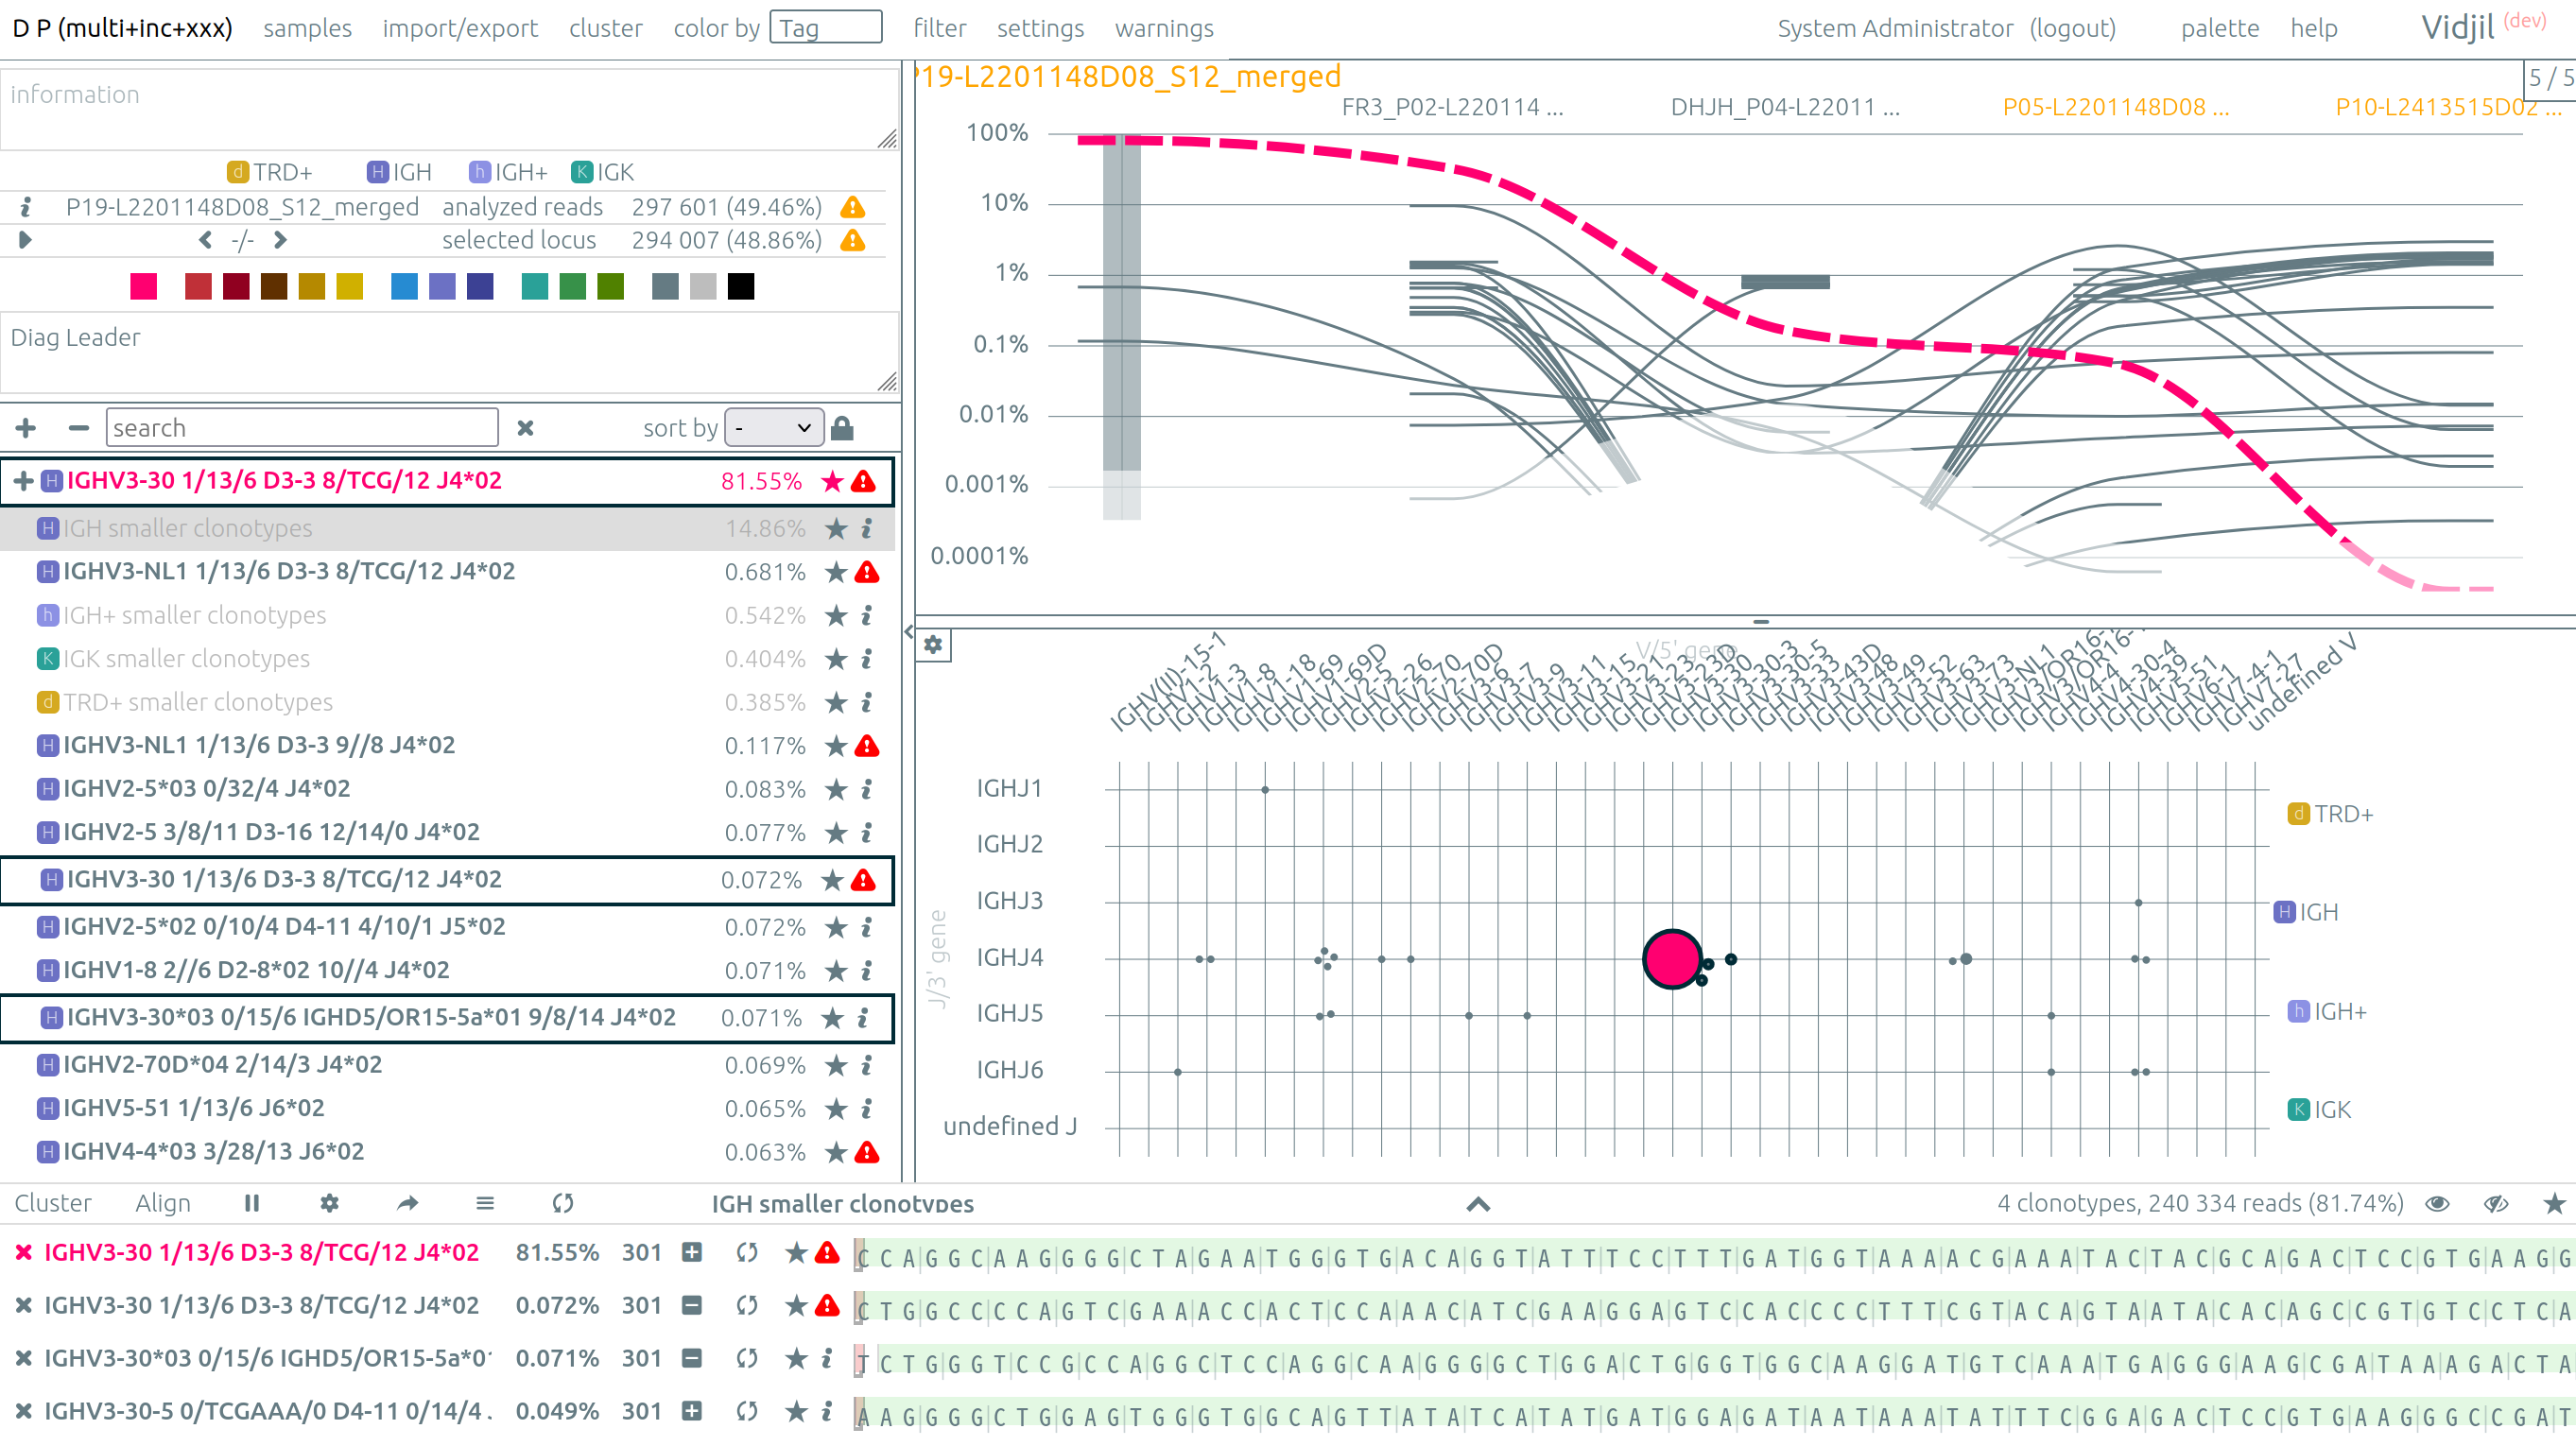
\includegraphics[width=1\textwidth]{images/vidjil-web.png}
    \caption{Interface de la plateforme web \textit{Vidjil}. 
    Liste des clones identifiés à gauche, visualisation de la cinétique des clones en haut à gauche, 
    familles \gls{vdj} en bas à droite, et séquences des clones sélectionnés en bas.}
    \label{fig:vidjil-web}
\end{figure}

\section{Applications en oncohématologie}

L'analyse du répertoire des gènes \gls{vdj} est particulièrement utile en oncohématologie, 
où la quasi unicité de chaque réarrangement \gls{vdj} peut servir de marqueur clonal hautement 
spécifique de certaines cellules tumorales et ainsi permettre leur détection et leur suivi \cite{hultcrantzBaselineVDJClonotype2020}.

\vspace{1em}
 
Avant toute chose, il peut être utile de dresser un panorama rapide des hémopathies malignes afin de 
mieux comprendre l'importance de l'analyse du répertoire des gènes \gls{vdj} dans ces situations.  
Ces pathologies regroupent ce qu'on appelle communément les « cancers du sang » et peuvent se séparer selon
leur origine en quatre grandes catégories. Une première séparation peut être établie entre les hémopathies 
myéloïdes et lymphoïdes selon l'origine des cellules. Brièvement, les cellules du sang et de la moelle sont soit de 
lignée lymphoïde pour les lymphocytes (B, T, NK et autres non conventionnels) et précurseurs, soit de lignée myéloïde 
pour le reste des cellules (hématies, plaquettes, polynucléaires, monocytes) et leurs précurseurs. Une seconde séparation 
est établie selon la maturité des cellules : on parle alors de \glspl{lam} et de \glspl{lal} lorsque la cellule 
tumorale dérive d'un précurseur, et de \glspl{smp} et de \glspl{slp}/\glspl{lnh} lorsque la cellule est mature (\autoref{fig:hemopathies}) 
\cite{alaggio5thEditionWorld2022a, khoury5thEditionWorld2022}.

\begin{figure}[H]
    \centering
    \begin{tikzpicture}[scale=1, every node/.style={font=\small}]

    \filldraw[fill=violet!30, opacity=0.2] (-2.5,0) rectangle (3,4); 
    \filldraw[fill=violet!60, opacity=0.4] (-2.5,-4) rectangle (3,0); 
    \filldraw[fill=blue!30, opacity=0.2] (3,0) rectangle (8.5,4); 
    \filldraw[fill=blue!60, opacity=0.4] (3,-4) rectangle (8.5,0);

    \node[rotate=90] at (-3,2) {Précurseurs (immature)};
    \node[rotate=90] at (-3,-2) {Cellules matures};
    \node at (0,4.3) {Myéloïde};
    \node at (6,4.3) {Lymphoïde};

    \node at (0,3.5) {\small \textbf{\gls{lam}}};
    \node at (6,3.5) {\small \textbf{\gls{lal}}};
    \node at (0,-0.5) {\small \textbf{\gls{smp}}};
    \node at (4.7,-0.5) {\small \textbf{\gls{slp}}};
    \node at (7,-0.5) {\small \textbf{\gls{lnh}}};

    \node at (0,1.7) {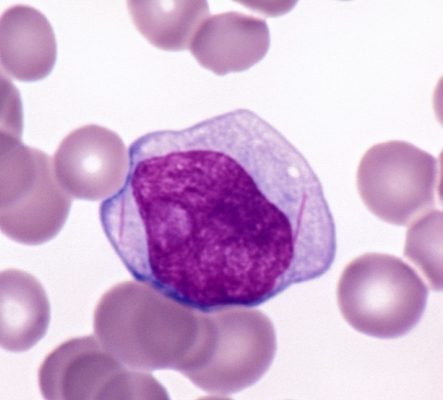
\includegraphics[width=3cm]{images/lam.jpg}};
    \node at (6,1.7) {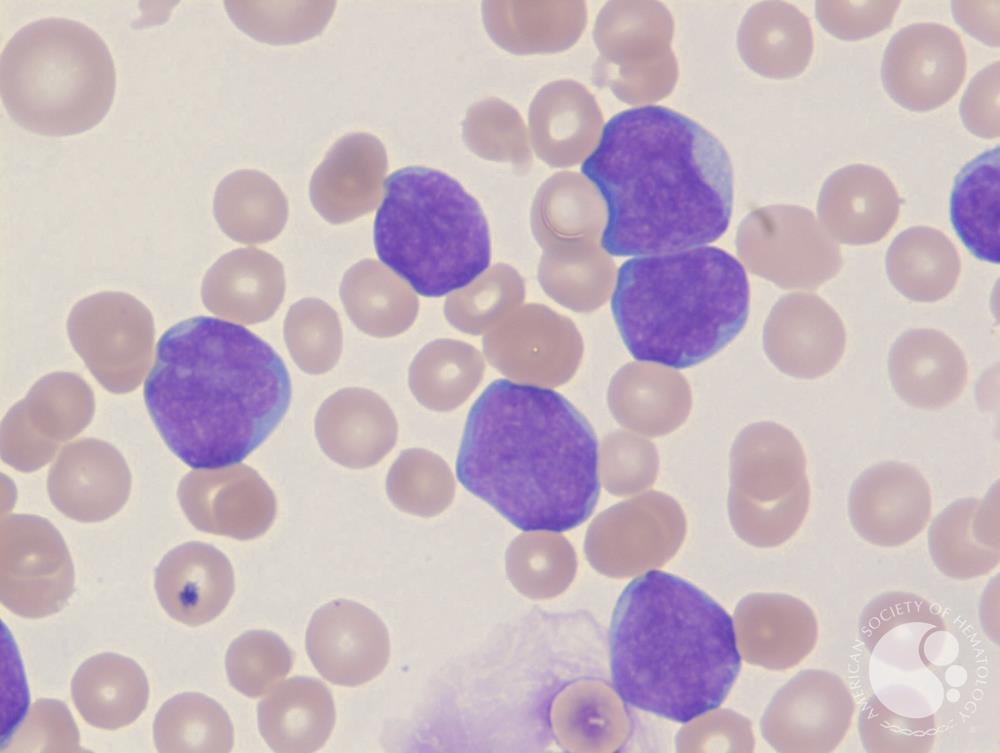
\includegraphics[width=3cm]{images/lal.jpeg}};
    \node at (-1,-2) {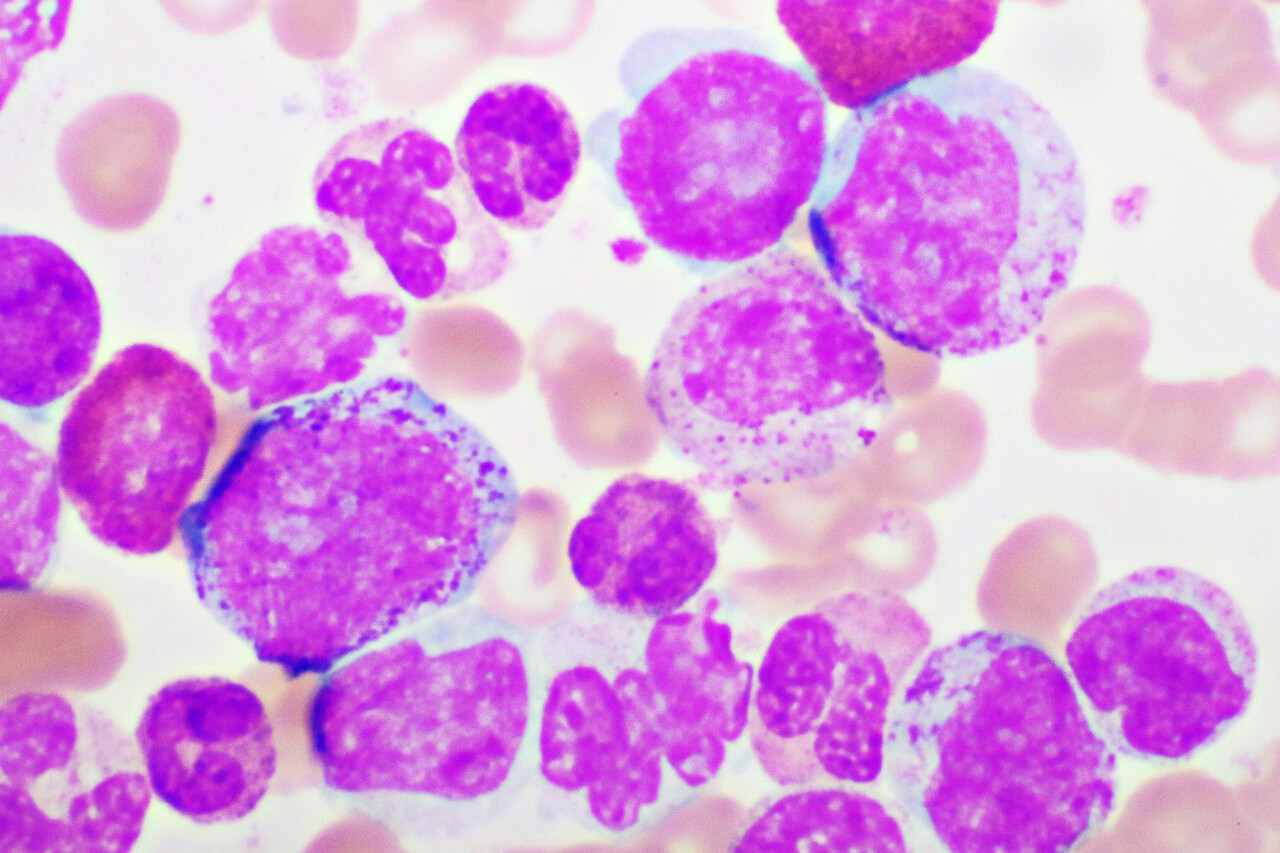
\includegraphics[width=2cm]{images/lmc.jpg}};
    \node at (1.2,-3) {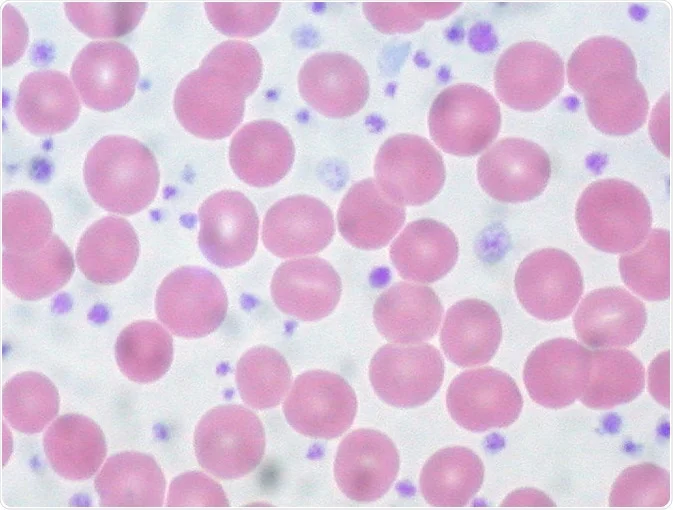
\includegraphics[width=2cm]{images/te.png}};
    \node at (4.7,-2) {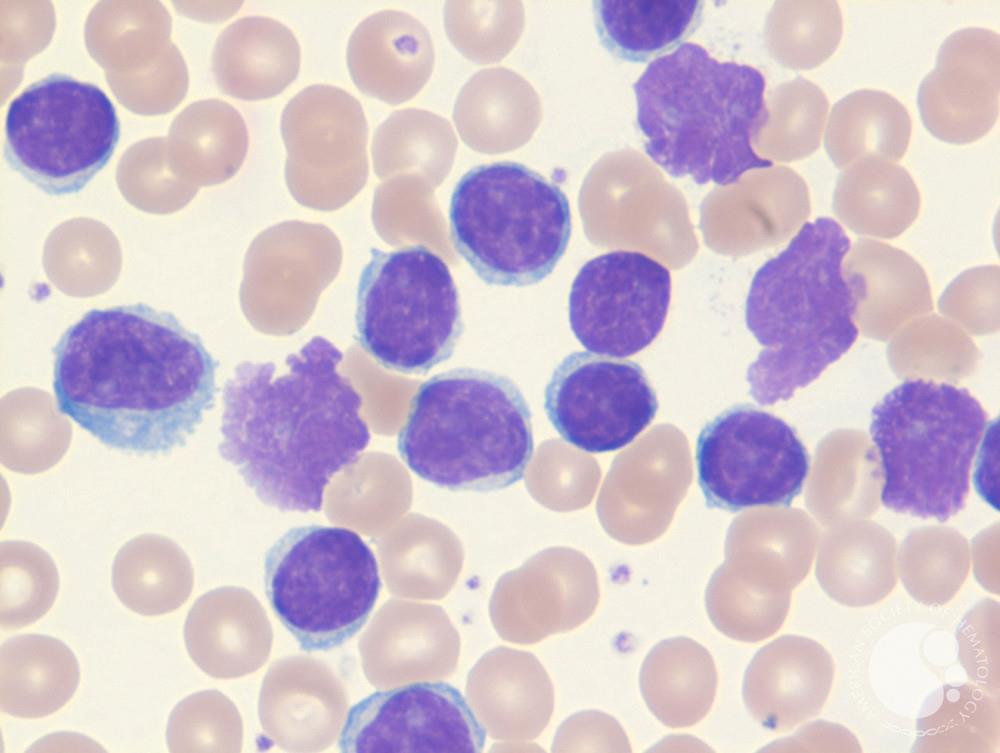
\includegraphics[width=2cm]{images/llc.jpeg}};
    \node at (7, -3) {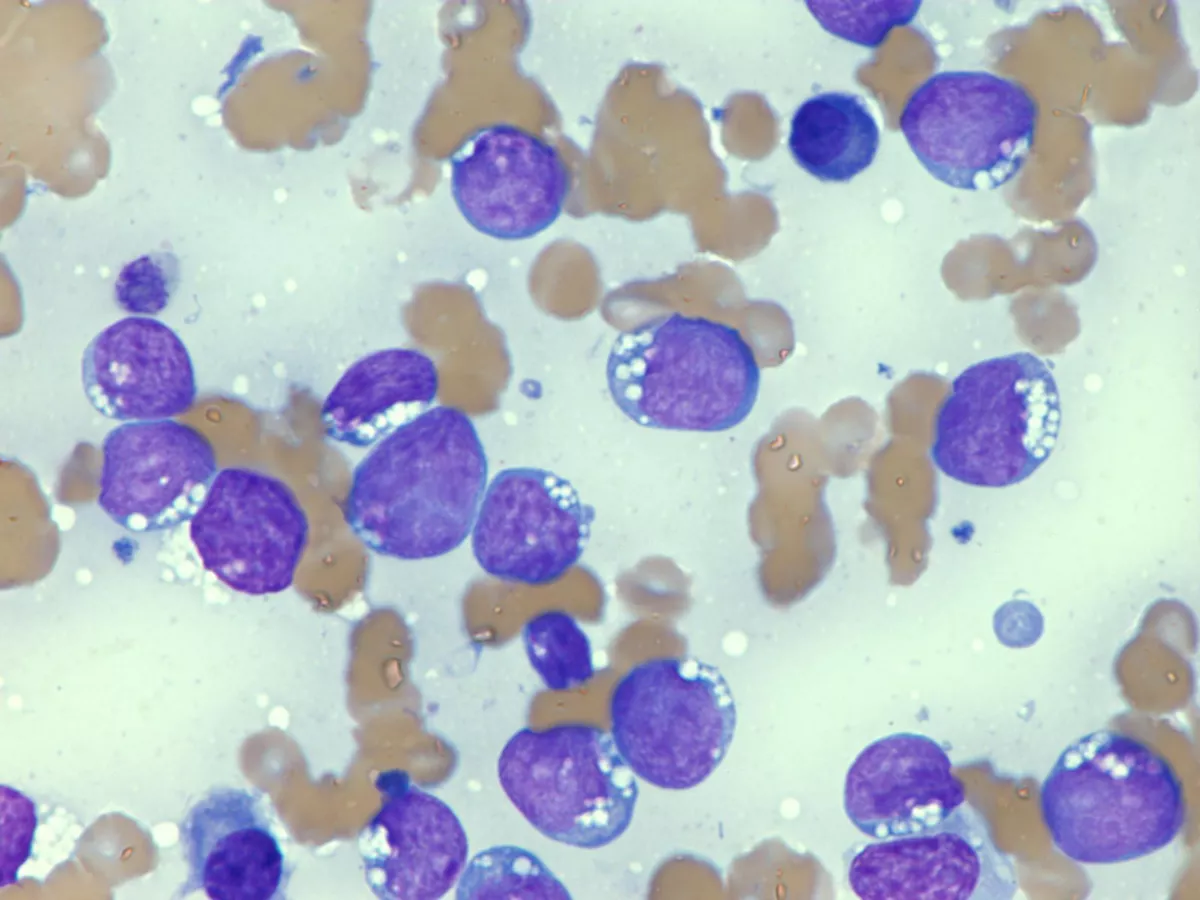
\includegraphics[width=2cm]{images/burkitt.png}};

    \draw[thick] (3,4.5) -- (3,-4.5); 
    \draw[thick] (-3,-0) -- (9,-0); 

    \end{tikzpicture}
    \caption{Classification des hémopathies malignes selon la lignée (myéloïde vs lymphoïde) 
    et le degré de maturité cellulaire (précurseur vs mature).}
    \label{fig:hemopathies}
\end{figure}


Dès lors \textit{Vidjil} trouve son utilité dans les hémopathies lymphoïdes, principalement dans les \glspl{lal} et les 
\glspl{llc} où il permet l'identification des réarrangements \gls{vdj} des \glspl{ig} et des \glspl{tcr} à des fins diverses.
Par exemple, dans les \glspl{llc} il permet d'identifier et d'annoter le segment V du réarrangement \textit{\gls{igh}} du clone tumoral, pour 
ensuite étudier le taux de mutations face aux séquences germinales, servant de marqueur pronostique fort de la pathologie
\cite{crombieIGHVMutationalStatus2017}.

\vspace{1em}

Dans le cadre de ce travail, nous nous sommes intéressés à une pathologie en particulier : le \gls{mm}, que l'on peut rattacher
au groupe des hémopathies lymphoïdes matures. Cette pathologie se caractérise par une prolifération maligne de plasmocytes, cellules
dérivées des lymphocytes B, responsables de la production et de la sécrétion des \glspl{ig} (anticorps) \cite{briglePathobiologyDiagnosisMultiple2017}. 
Elles constituent le stade le plus mature de la lymphopoïèse B, à la suite de la différenciation des lymphocytes B naïfs 
au contact de l'antigène, et sont les principaux acteurs de la réponse immunitaire humorale adaptative.

\vspace{1em}

Dans le \gls{mm}, les plasmocytes malins prolifèrent de manière incontrôlée, entraînant une altération du fonctionnement normal de la moelle osseuse,
avec des anémies, un déficit immunitaire secondaire, des atteintes osseuses, et une insuffisance rénale. Une partie de ces symptômes est causée
par la production d'une \gls{ig} monoclonale, dont la détection par électrophorèse constitue un élément diagnostique majeur, au même titre que la
prolifération médullaire des plasmocytes malins et les autres signes cliniques et biologiques précédemment décrits \cite{cowanDiagnosisManagementMultiple2022a} 
(\autoref{fig:mm-cells-ig}).

\begin{figure}[H]
    \begin{minipage}{0.45\textwidth}
        \centering
        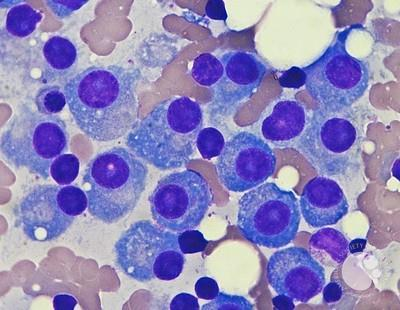
\includegraphics[width=1\textwidth]{images/mm_cells.jpeg}
    \end{minipage}
    \hfill
    \begin{minipage}{0.45\textwidth}
        \centering
        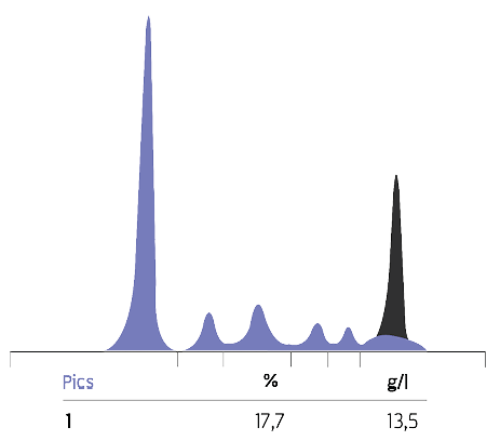
\includegraphics[width=01\textwidth]{images/pic.png}
    \end{minipage}
    \caption{Gauche : Prolifération de plasmocytes malins dans la moelle osseuse. 
    Droite : Electrophorèse des protéines sériques montrant la présence d'une \gls{ig} monoclonale (pic noir) 
    superposée à un profil normal en bleu.}
    \label{fig:mm-cells-ig}
\end{figure}

Le myélome multiple touche majoritairement les personnes âgées, avec un âge médian au diagnostic d'environ 70 ans. Il représente environ 10 \%
des hémopathies malignes et près de 1 \% de l'ensemble des cancers. En France, on estime à environ 6 000 le nombre de nouveaux cas chaque année 
\cite{spfSurviePersonnesAtteintes}.

\vspace{1em}

Sur le plan thérapeutique, les stratégies ont considérablement évolué ces dernières années. Le traitement repose sur une approche personnalisée
selon l'âge et l'état général du patient. Chez les patients éligibles, une chimiothérapie d'induction est souvent suivie d'une autogreffe de cellules
souches hématopoïétiques. Chez les patients plus âgés ou fragiles, des protocoles associant agents immunomodulateurs (tels que la lénalidomide),
inhibiteurs du protéasome (comme le bortézomib) et anticorps monoclonaux (notamment l'anti-CD38, daratumumab) sont privilégiés. Le traitement de
maintenance et la surveillance à long terme permettent de prolonger la réponse et de retarder les rechutes, fréquentes dans cette pathologie chronique 
\cite{cowanDiagnosisManagementMultiple2022a}.

\vspace{1em}

En ce qui concerne le \gls{mm}, l'intérêt de l'analyse du répertoire \gls{vdj} se rapproche de celui des \glspl{lal} où l'identification 
de réarrangement \gls{vdj} (en l'occurrence ici des \textit{\gls{igh}} ou des \textit{\gls{igk}} et \textit{\gls{igl}}) sert de marqueur unique (dit de clonalité) 
de la cellule tumorale, et permet ainsi de suivre l'évolution de la maladie.

\section{Maladie résiduelle et ADN circulant tumoral}

Comme de nombreuses autres hémopathies, le \gls{mm} est une pathologie dont l'évolution clinique peut être très hétérogène. 
Si certaines caractéristiques observées au diagnostic permettent de dresser un pronostic plus ou moins favorable, 
la trajectoire de la maladie reste souvent difficile à prédire \cite{hanamuraMultipleMyelomaHighrisk2022}. 
Dans ce contexte, un marqueur particulièrement pertinent de l'évolution de la maladie et de la réponse au traitement 
est la présence d'une \gls{mrd} dite indétectable.

\vspace{1em}

La \gls{mrd} désigne la persistance de cellules tumorales résiduelles non détectables 
par les méthodes conventionnelles (telles que l'analyse morphologique ou biochimique), mais que l'on peut mettre en évidence 
grâce à des techniques de haute sensibilité, comme la \gls{cmf} multiparamétrique ou la biologie moléculaire. Elle représentent 
en quelque sorte la « face cachée de l'iceberg » de la maladie, qui persiste même lorsque les signes cliniques et biologiques 
ont disparu (\autoref{fig:mrd-techniques}).
Dans le cas spécifique du \gls{mm}, l'évaluation de la \gls{mrd} repose souvent sur la détection de cellules présentant des 
aberrations phénotypiques par \gls{cmf} ou sur la détection de réarrangements \gls{vdj} propres au clone tumoral, permettant un suivi très ciblé 
mais plus complexe à mettre en oeuvre \cite{bertaminiMRDAssessmentMultiple2021}.

\begin{figure}[H]
    \centering
    \begin{tikzpicture}

    % iceberg
    \node at (0,0.8) {
\includegraphics[width=10cm]{images/iceberg.jpg}}; 

    % seuils
    \draw[dashed] (-3.5,2.5) -- (3.5,2.5);
    \draw[dashed] (-3.5,-0.5) -- (3.5,-0.5);
    \draw[dashed] (-3.5,-2) -- (3.5,-2);

    \node at (0,3.2) {\textbf{Maladie à expression clinique}};
    \node at (0,0.8) {\textbf{\gls{mrd}}};
    \node at (0,-1.4) {\textbf{\gls{mrd} non quantifiable}};
    \node at (0,-3) {\textbf{Maladie non détectable}};

    % axe cellules leucémiques 
    \draw[very thick] (-3.5,4.2) -- (-3.5,-4.2);
    \node[rotate=90] at (-4.5,0) {Nombre de cellules leucémiques};

    \node at (-3.9,4.0) {$10^{12}$};
    \node at (-3.9,2.5) {$10^{10}$};
    \node at (-3.9,1) {$10^{8}$};
    \node at (-3.9,-0.5) {$10^{6}$};
    \node at (-3.9,-2) {$10^{4}$};
    \node at (-3.9,-3.5) {$10^{2}$};

    % axe valeurs de mrd
    \draw[very thick] (3.5,4.2) -- (3.5,-4.2);
    \node[rotate=-90] at (4.7,0) {Valeurs de \gls{mrd}};

    \node at (4,2.5) {$10^{-2}$};
    \node at (4,1) {$10^{-4}$};
    \node at (4,-0.5) {$10^{-6}$};
    \node at (4,-2) {$10^{-8}$};
    \node at (4,-3.5) {$10^{-10}$};

    % Techniques de détection
    \node[align=center, text width=4cm, font=\bfseries] at (7,4.4) {Méthodes de mesure};

    \node[anchor=west] at (5.5,3.3) {
\includegraphics[width=1.5cm]{images/microscope.png}};
    \node[anchor=west] at (7.8,3.3) {Microscopie optique};

    \node[anchor=west] at (5.5,1.5) {
\includegraphics[width=1.5cm]{images/cmf.png}};
    \node[anchor=west] at (7.8,1.5) {\gls{cmf}};

    \node[anchor=west] at (5,0) {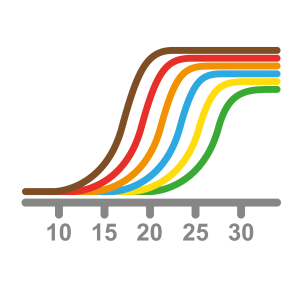
\includegraphics[width=1.5cm]{images/pcr.png}};
    \node[anchor=west] at (7.8,0) {\gls{pcr} quantitative};

    \node[anchor=west] at (6.2,-0.5) {
\includegraphics[width=1.5cm]{images/ngs.png}};
    \node[anchor=west] at (7.8,-0.5) {\gls{hts}};

    \node[align=center] at (7.5,-2.5) {\gls{mrd} non détectable \\ avec les méthodes actuelles};
    \node[align=center] at (7.5,-3.5) {\textbf{Guérison}};

    \end{tikzpicture}
    \caption{
    Représentation schématique des techniques de détection de la \gls{mrd} et des seuils de détection en 
    regard du nombre de cellules leucémiques.
    Les techniques de détection sont classées selon leur sensibilité, allant de la morphologie à la biologie 
    moléculaire. Adapté de \citeauthor{sayginMeasurableResidualDisease2022} \cite{sayginMeasurableResidualDisease2022}.
    }
    \label{fig:mrd-techniques}
\end{figure}



L'intérêt pronostique de la \gls{mrd} a largement été démontré dans d'autres hémopathies malignes, notamment dans les \gls{lal} et \gls{lam}, 
où elle s'est imposée comme un outil essentiel pour guider et adapter les stratégies thérapeutiques. Dans le \gls{mm}, l'absence de \gls{mrd} 
après traitement est également associée à une durée de rémission prolongée et à une survie globale améliorée. A l'inverse, une \gls{mrd} détectable, 
même à très faible niveau, constitue un facteur de risque important de rechute précoce (\autoref{fig:mrd})
\cite{munshiLargeMetaanalysisEstablishes2020}.

\vspace{1em}

Ainsi, le suivi de la \gls{mrd} tend aujourd'hui à devenir non seulement un critère d'évaluation de l'efficacité thérapeutique, mais aussi un objectif 
thérapeutique propre dans le \gls{mm}. De plus en plus d'essais cliniques intègrent désormais la \gls{mrd} comme critère principal d'évaluation, 
voire comme élément décisionnel pour intensifier, adapter ou interrompre un traitement.

\begin{figure}[H]
    \centering
    \begin{tikzpicture}
    \begin{semilogyaxis}[
        width=14cm,
        height=8cm,
        xlabel={Temps (unité arbitaire)},
        ylabel={Proportion de cellules leucémiques},
        ymin=1e-7, ymax=1,
        ytick={1e0,1e-1,1e-2,1e-3,1e-4,1e-5,1e-6},
        yticklabels={$10^{0}$,$10^{-1}$,$10^{-2}$,$10^{-3}$,$10^{-4}$,$10^{-5}$,$10^{-6}$},
        xtick=\empty,
        axis lines=left,
        grid=none,
        clip=false,
    ]

    % sections d'arrière plan
    \addplot [draw=none, fill=red!10]
     coordinates {
        (0,1e0) (10,1e0) (10,5e-2) (0,5e-2)
    } -- cycle;

    \addplot [draw=none, fill=orange!10
    ] coordinates {
        (0,5e-2) (10,5e-2) (10,1e-4) (0,1e-4)
    } -- cycle;

    \addplot [draw=none, fill=green!10
    ] coordinates {
        (0,1e-4) (10,1e-4) (10,1e-7) (0,1e-7)
    } -- cycle;

    % lignes horizontales pour les seuils
    \foreach \y in {1e-1,1e-2,1e-3,1e-4,1e-5} {
        \addplot[dashed, color=black!60] coordinates {(0,\y) (10,\y)};
    }

    % réponse complète avec MRD-
    \addplot[thick, red, smooth] coordinates {
        (0,5e-1) (1,1e-3) (2,5e-3) (3,1e-2) (4,5e-2) (5,1e-1) (6,9e-1)
    };

    % rechute précoce
    \addplot[thick, blue, smooth] coordinates {
        (0,5e-1) (1,1e-3) (2,1e-4) (3,1e-5) (4,5e-6) (5,1e-6) (6,1e-6) (7,1e-6) (8,1e-6)
    };

    % rechute moléculaire 
    \addplot[thick, violet, smooth] coordinates {
        (0,7e-1) (1,1e-2) (2,5e-3) (3,1e-4) (4,5e-5) (5,5e-6) (6,1e-4) (7,1e-3) (8,1e-2)
    };

    % labels
    \node[align=left, anchor=west, blue!50!black] at (axis cs:6,2e-6) {réponse complète avec MRD-};
    \node[align=left, anchor=west, violet!50!black] at (axis cs:7,2e-2) {rechute moléculaire};
    \node[align=center, anchor=south east, red!50!black] at (axis cs:5,1e-1) {rechute hématologique précoce};

    \end{semilogyaxis}
    \end{tikzpicture}
    \caption{Suivi de la \gls{mrd} dans le temps. Exemple de trois réponses différentes selon le statut 
    de la \gls{mrd} : \textcolor{blue}{réponse complète avec \gls{mrd}- en bleu},  
    \textcolor{red}{rechute précoce en rouge} et \textcolor{violet}{rechute moléculaire en violet}.}
    \label{fig:mrd}
\end{figure}


Pour autant, l'analyse de la \gls{mrd} pose certaines difficultés, notamment en ce qui concerne la sensibilité et la spécificité des techniques utilisées.
Il faut pouvoir être en mesure de détecter un nombre extrêmement faible de cellules tumorales parmi une population très majoritaire de cellules normales,
ce qui exige des méthodes à très haut pouvoir résolutif et des échantillons de qualité et quantité suffisante.

\vspace{1em}

La \gls{cmf}, bien qu'accessible dans de nombreux centres, dépend fortement de l'expertise technique et de la standardisation
des panels d'anticorps utilisés. De plus, son seuil de détection, généralement de l'ordre de $10^{-3}$ à $5.10^{-5}$, peut s'avérer insuffisant dans certains contextes
thérapeutiques.

\vspace{1em}

Les approches moléculaires, comme le \gls{ngs} ciblant les réarrangements \gls{vdj}, offrent une sensibilité encore plus élevée (jusqu'à $10^{-6}$),
mais nécessitent une connaissance préalable du profil clonotypique du patient, ainsi qu'un accès à des plateformes technologiques spécialisées et solutions 
bioinformatiques dédiées. Par ailleurs, s'agissant du \gls{mm}, la détection des réarrangements \gls{vdj} peut être compliquée par la présence de nombreuses 
mutations sur la région V des \glspl{ig} à la suite du phénomène d'hypermutation somatique, ce qui peut rendre difficile l'amplification des séquences.

\vspace{1em}

Enfin, la représentativité de l'échantillon, souvent issu d'une ponction médullaire unique, peut aussi poser problème en raison de la distribution hétérogène
des plasmocytes tumoraux dans la moelle osseuse. Cette variabilité peut conduire à une sous-estimation de la \gls{mrd} en cas de prélèvement non représentatif.
Par ailleurs, la nécessité de prélèvements médullaires peut également constituer un frein à l'évaluation répétée de la \gls{mrd}, du fait de leur caractère
invasif, et souvent inconfortable pour le patient.

\vspace{1em}

Dans ce contexte, l'analyse des acides nucléiques circulants, et en particulier de l'\gls{adnc}, suscite un intérêt croissant. Ces fragments d'ADN, libérés dans le sang 
par les cellules tumorales et normales en apoptose ou en nécrose, peuvent refléter de manière globale la charge tumorale et permettre une évaluation non 
invasive de la \gls{mrd} (\autoref{fig:ctdna}). Contrairement à la ponction médullaire, un simple prélèvement sanguin (ou « biopsie liquide ») permet de suivre plus facilement 
et plus fréquemment l'évolution de la maladie.

\vspace{1em}

Bien que cette approche soit largement démocratisée dans le domaine de l'oncologie solide, elle reste encore en cours de validation en oncohématologie et demeure,
pour le moment, marginale, avec quelques applications dans le cadre des \glspl{lnh}. Dans les autres pathologies, les défis techniques liés à la faible concentration des 
\gls{adnc} et à la faible taille des fragments ($\approx$ 150 pb), à l'hétérogénéité génétique des hémopathies malignes et à l'absence de biomarqueurs universels 
limitent encore son déploiement en routine clinique \cite{daoUsingCfDNACtDNA2023}.

\begin{figure}[H]
    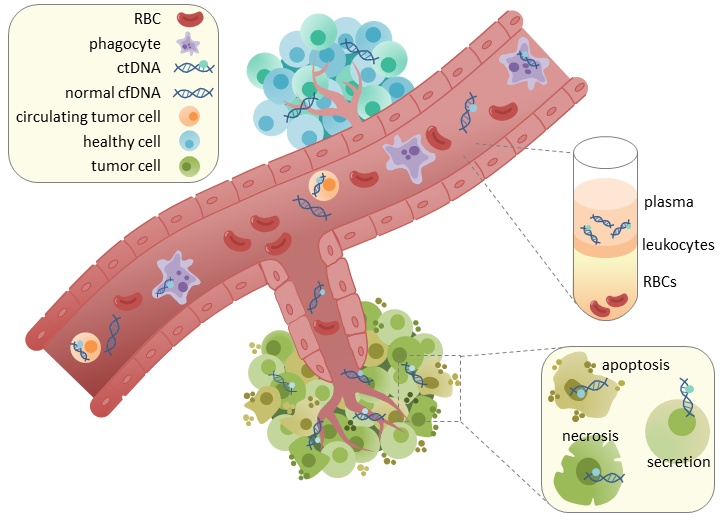
\includegraphics[width=1\textwidth]{images/ctdna.png}
    \caption{Origines des \gls{adnc}. \citeauthor{racheljunewongEnglishCirculatingTumor2017} \cite{racheljunewongEnglishCirculatingTumor2017}.}
    \label{fig:ctdna}
\end{figure}
    


\chapter{Problématique et objectifs}

Ainsi, l'objectif de ce travail a été de développer un protocole d'analyse via
\textit{Vidjil} pour l'étude de la \gls{mrd} dans le \gls{mm}. Dans un premier
temps, l'objectif a été de mettre en place un protocole reproductible
permettant d'identifier les réarrangements clonaux à partir d'ADN génomique,
extrait de prélèvements médullaires. Cette phase a servi de référence pour
caractériser le réarrangement \gls{vdj} dominant propre à chaque patient, et
constituer une signature clonale utilisable pour le suivi ultérieur, sur ADN
génomique et \gls{adnc}.

\vspace{1em}

Dans un second temps, l'objectif (bien que non atteint à ce jour, mais qui aura
guidé les décisions entreprises) était de rechercher ces réarrangements dans
l'\gls{adnc} issu de prélèvements sanguins. L'analyse de ce type d'échantillons
soulève plusieurs défis techniques et bioinformatiques : d'une part, la très
faible concentration d'\gls{adnc} dans le plasma nécessite des méthodes de
quantification sensibles et fiables ; d'autre part la fragmentation naturelle
du \gls{adnc}, rend plus difficile l'identification des réarrangements clonaux,
souvent de l'ordre de 500 pb contre seulement 150 pb pour l'\gls{adnc}.

\vspace{1em}

Un autre pan de ce travail a également consisté à adapter l'analyse faite par
\textit{Vidjil} à ces spécificités, en évaluant la pertinence des paramètres de
détection utilisés par \textit{Vidjil} pour l'\gls{adnc} (ou l'ADN génomique
traité comme tel) et en développant des outils de traitement personnalisés pour
l'exploration des résultats.

\vspace{1em}
% toujours un peu de mal avec le terme sensibilité ... Tu ne penses pas que LOD
% c'est mieux ?

Enfin, une étude des performances analytiques du protocole a été menée, avec
une attention particulière portée à la sensibilité (détection de faibles taux
de \gls{mrd}) et à la spécificité (éviction des signaux non clonaux ou
artefactuels), afin d'évaluer la faisabilité de cette approche dans un
environnement clinique pour le suivi thérapeutique.


\chapter{Matériels et Méthodes}

\section{Echantillons biologiques}

Les prélèvements sont issus d'une collaboration directe avec le laboratoire d'hématologie et la tumorothèque du 
\gls{chu} (GCS-ALLIANCE CANCER). Des échantillons de moelle osseuse et de sang périphérique de patients 
atteints de \gls{mm} et \gls{llc} ont été requalifiés à visée de recherche par le comité scientifique (n° d'avis CSTMT350 \autoref{anx:cstmt-mrd-mm}). 
Ces prélèvements ont été utilisés lors des étapes de mise au point technique. Par la suite 5 couples de prélèvements 
au diagnostic et au suivi de patients traités pour un \gls{mm} ont été sélectionnés pour l'analyse de la \gls{mrd}. Pour ces 
prélèvements, l'histoire clinique ainsi que la \gls{mrd} évalée par \gls{cmf} sont disponibles.

\section{Préparation et séquençage haut-débit}

Les échantillons de moelle osseuse et de sang périphérique sont traités selon les procédures standards du laboratoire 
d'hématologie : les prélèvements au diagnostic subissent un tri magnétique CD138+ pour isoler les plasmocytes puis l'ADN 
est extrait et cryopréservé. Pour les prélèvements au suivi, l'ADN est extrait directement à partir du culot cellulaire 
après lyse des hématies.

\vspace{1em}

La préparation de la librairie de séquençage est réalisée en une seule étape de \gls{pcr} via des amorces contenant les 
régions spécifiques à amplifier, les adaptateurs pour le séquençage et les codes-barres pour l'identification des échantillons 
(\autoref{anx:primer-sequences}).

\vspace{1em}

En raison de l'objectif d'analyser \textit{in fine} des échantillons d'\gls{adnc} qui, comme vu précédemment sont de petite taille, 
les amorces choisis ciblent la région \gls{fr}3 (cf \autoref{fig:igh}) des gènes \textit{\gls{igh}} pour pouvoir séquencer l'ensemble de la 
région \gls{cdr}3 porteuse de l'unicité du réarrangement. 
Ces amorces sont adaptées des recommandations du groupe européen de l'EuroClonalité \cite{langerakEuroClonalityBIOMED2Guidelines2012} 
et modifiées pour l'amplification d'\gls{adnc} par \citeauthor{pottCfDNABasedNGSIG2022a} \cite{pottCfDNABasedNGSIG2022a}.
Un standard interne (\textit{spike-in}) titré à $10^{-4}$ cellules est ajouté pour corriger les biais de séquençage en vue de la quantification 
pour les prélèvements au suivi. En parallèle, l'ADN du diagnostic est également utilisé dilué à $10^{-4}$ pour l'étude de la limite de détection. 
L'ADN amplifié est ensuite purifié sur billes, analysé et dosé puis séquencé sur plateforme Illumina MiSeq en \textit{paired-end} 2x300 bases.

\section{Environnement d'analyse et de développement}

L'analyse des données de séquençage est réalisée dans un premier temps sur \textit{Vidjil}, via une machine virtuelle dédiée,
hébergée au \gls{chu}. Par la suite, une fois les données anonymisées, elles sont transférées sur un environnement de 
développement Ubuntu 24.04.2 LTS (autrement dit, un ordinateur personnel) pour la mise au point de l'analyse de la \gls{mrd}.
\textit{Vidjil} est utilisé dans sa version 2024.02 pour \textit{vidjil-algo} et \texttt{release} 2024.12 puis 2025.06 pour la partie 
web. La configuration d'analyse utilisée est \textit{multi+inc+xxx} permettant la detection multi loci des recombinaisons complètes, 
incomplètes, atypiques et inattendues.
L'ensemble des modifications et développements réalisés sur \textit{Vidjil} concerne la partie client, et dans une moindre mesure,
la partie serveur. Elles sont consultables sur le dépôt \href{https://gitlab.inria.fr/users/x-benha/activity}{\textit{GitLab}}
de \textit{Vidjil}, et sont documentées dans les requêtes de fusion \href{https://gitlab.inria.fr/vidjil/vidjil/-/merge_requests/1610}{1610}
et \href{https://gitlab.inria.fr/vidjil/vidjil/-/merge_requests/1631}{1631} associées.


\chapter{Résultats}

\section{Premier essai}

\subsection{}
\chapter{Travaux effectués au CHU de Lille}

Cette section, bien que légèrement en marge du reste du rapport, a pour objectif de présenter un bref aperçu 
de plusieurs projets réalisés durant la seconde moitié de ce stage, au sein de l'équipe bioinformatique du \gls{chu}, 
principalement en lien avec le \gls{mm}. Ces projets portent essentiellement sur la gestion des pipelines d'analyse 
des données de séquençage, comprenant la création d'un nouveau pipeline, l'ajout d'une fonctionnalité spécifique à 
un pipeline existant, ainsi que la mise à jour et la rédaction de tests pour trois autres pipelines. Parallèlement, 
la gestion des cycles de qualification et de production a été assurée. Cette section a été encadrée par Augustin Boudry du \gls{chu}.

\section{Architecture logicielle et environnement utilisateur}

L'environnement de développement du \gls{chu} s'appuie sur plusieurs composantes clés, côté développeur comme côté utilisateur.
Des machines virtuelles sous Rocky Linux 9.2 sont mises à disposition pour les développements et la routine d'analyse.
Elles sont hébergées sur un \gls{hpc} orchestré via \href{https://oar.imag.fr/}{OAR} et très récemment \href{https://slurm.schedmd.com/documentation.html}{Slurm},  
comprenant X Go de mémoire vive, X nœuds de calcul, deux serveurs GPU, ainsi qu'un serveur de stockage de X To.
Le gestionnaire de \textit{workflow} \href{https://www.nextflow.io/}{Nextflow} est utilisé pour l'écriture des différents pipelines d'analyse, 
déployés via une conteneurisation des dépendances dans des images \textit{Singularity} et de l'environnement dans des conteneurs \textit{Docker}.
De nombreuses surcouches logicielles sont développées par l'équipe afin de faciliter, automatiser et sécuriser les phases de développement et d'utilisation.
On peut citer notamment les \textit{nf-tools}, qui permettent d'automatiser un certain nombre de tâches, allant de la création des projets au lancement des pipelines.
Enfin, des interfaces web permettent d'accéder de façon simple à l'ensemble des applications développées par l'équipe (\autoref{fig:bioinfo-dashboard}).
L'ensemble du code est versionné et hébergé sur un dépôt GitLab interne au \gls{chu}.

schéma Augustin architecture ? 

\begin{figure}[H]
    \centering
    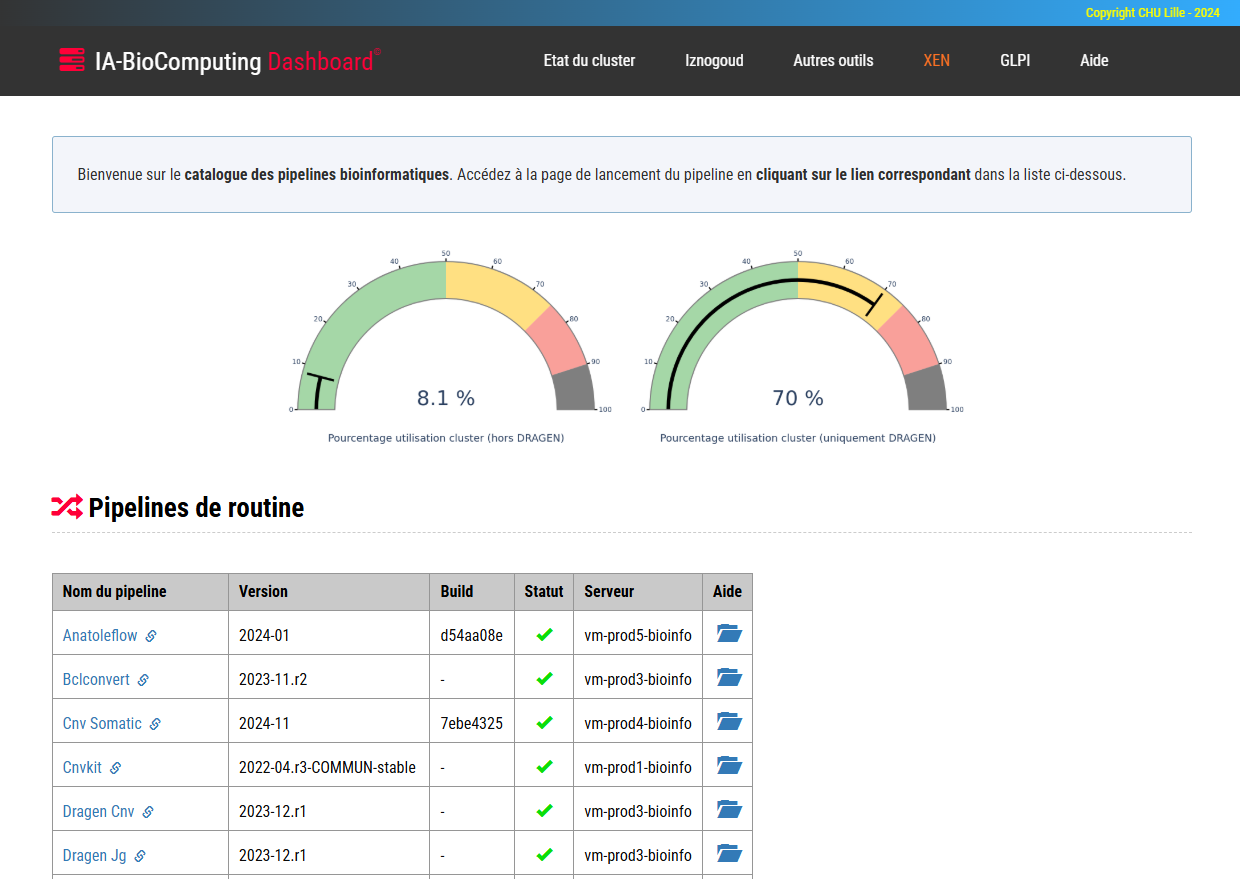
\includegraphics[width=1\textwidth]{images/dashboard_bioinfo.png}
    \caption{
        Page d'acceuil de lancement des pipelines et autres outils bioinformatiques du \gls{chu}.
    }
    \label{fig:bioinfo-dashboard}
\end{figure}

\section{Quantification des délétions du gène \textit{TP53}}

Ce rapport a principalement traité du suivi de la \gls{mrd} dans le \gls{mm}, une analyse à visée pronostique réalisée au cours du suivi des patients.
Plaçons-nous à présent dans une optique toujours pronostique (voire diagnostique) mais cette fois au moment du diagnostic de la pathologie. 
Trois analyses moléculaires sont alors réalisées :

\begin{itemize}
    \item \textbf{La recherche de variants somatiques} dans des gènes d'intérêt, notamment des oncogènes et des gènes suppresseurs de tumeurs.
    \item \textbf{La recherche de translocations} impliquant les \glspl{ig} et d'autres partenaires chromosomiques.
    \item \textbf{L'analyse du nombre de copies} permettant d'identifier des anomalies comme des duplications ou des délétions.
\end{itemize}

\vspace{1em}

C'est dans le cadre de cette dernière analyse qu'il a été nécessaire de développer une approche spécifique pour quantifier les délétions du gène \textit{TP53}, 
gène suppresseur de tumeur dont l'altération est associée à un mauvais pronostic dans le \gls{mm}, avec un seuil placé à 20 \% des cellules selon des recommandations 
récentes non publiées \cite{flyntPrognosisBiologyTargeting2020}.
Les plasmocytes étant des cellules particulièrement difficiles à cultiver, l'analyse du nombre de copies, associée aux techniques de \gls{fish} 
\footnote{La \gls{fish} est une technique de cytogénétique moléculaire permettant de détecter et localiser des séquences d'ADN spécifiques sur des chromosomes, à l'aide de sondes fluorescentes complémentaires. 
Elle est couramment utilisée pour identifier des anomalies chromosomiques, telles que des translocations, délétions ou amplifications.}, constitue l'unique 
moyen d'accéder aux remaniements génomiques de grande taille (duplications, délétions, translocations, etc.).
Ces informations permettent de dresser ce que l'on peut considérer comme un « carytoype moléculaire » de la cellule tumorale. 

\vspace{1em}

Il est aisé, grâce à la technique de \gls{fish}, de quantifier ce type d'événement en comptant directement le nombre de cellules portant l'anomalie parmi l'ensemble des cellules analysées 
(\autoref{fig:fish}).  
En revanche, il est beaucoup plus difficile d'estimer avec précision la fréquence de ces anomalies dans le cadre d'analyses en \textit{bulk}, comme celles réalisées par \gls{ngs}.

\begin{figure}[H]
    \begin{minipage}{0.45\textwidth}
        \centering
        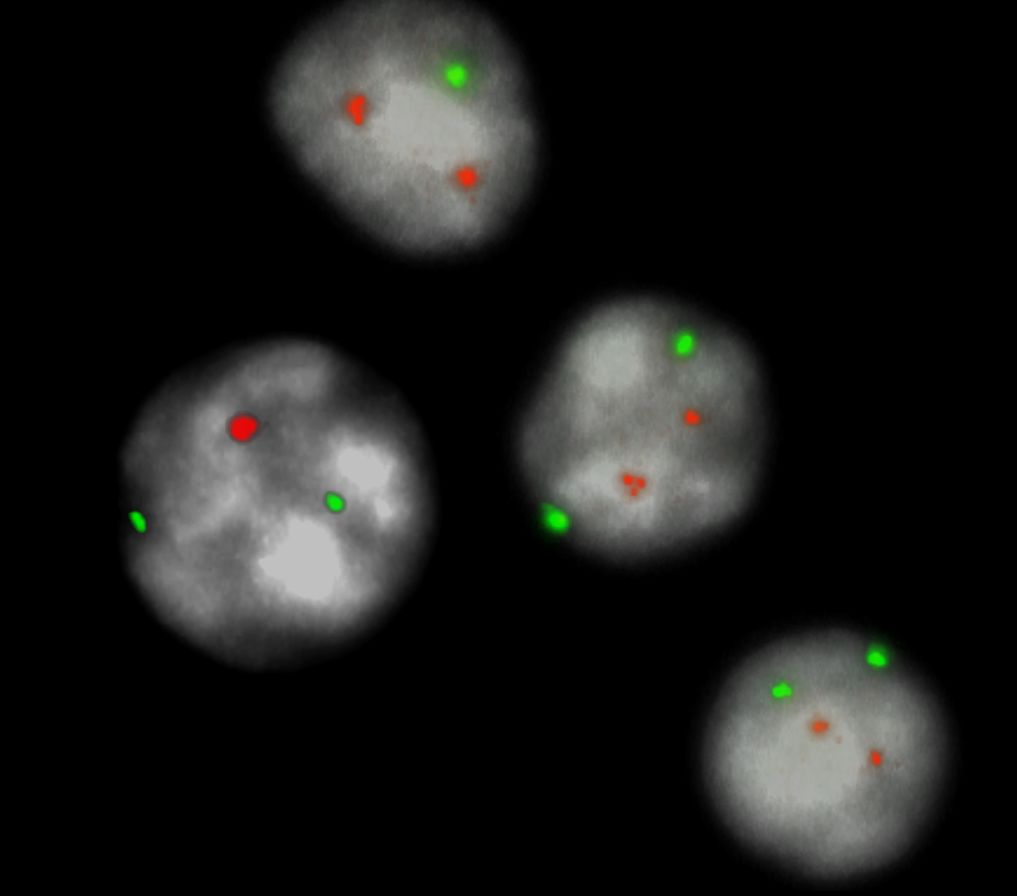
\includegraphics[width=1\textwidth]{images/fish_image.png}
    \end{minipage}
    \hfill
    \begin{minipage}{0.45\textwidth}
        \centering
        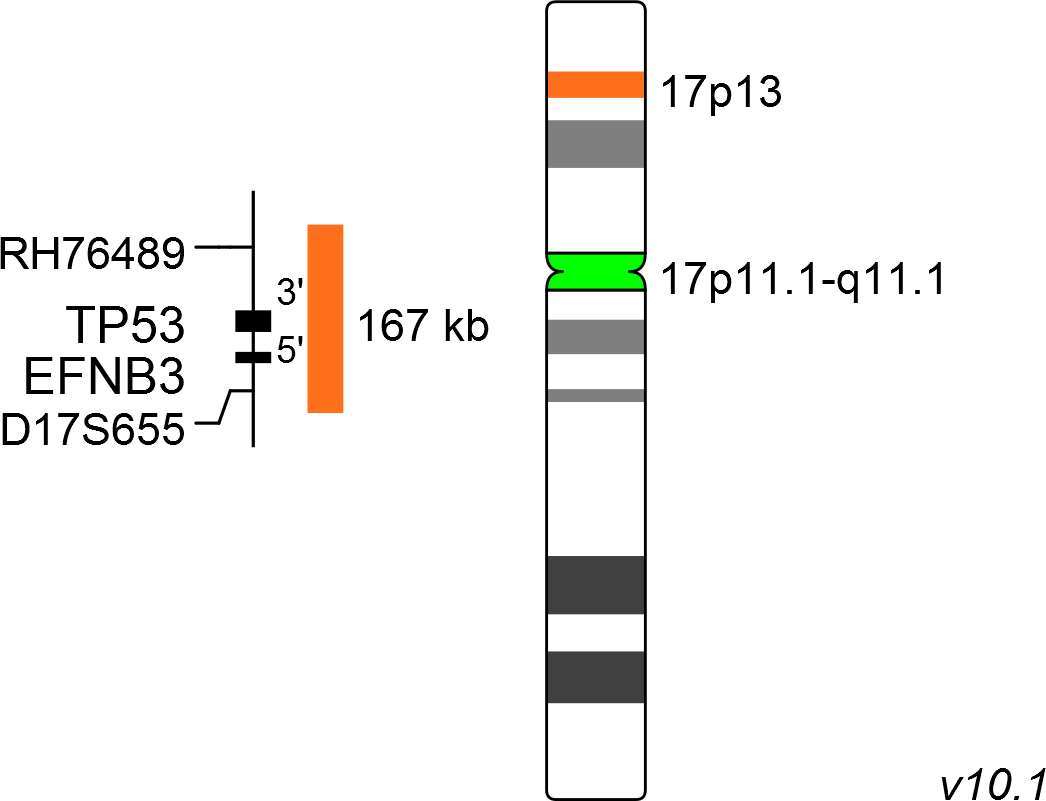
\includegraphics[width=01\textwidth]{images/fish.png}
    \end{minipage}
    \caption{
        \gls{fish} \textit{TP53} sur noyaux interphasiques à gauche et \textit{design} de la sonde à droite. 
    }
    \label{fig:fish}
\end{figure}

Pour des raisons internes au laboratoire, l'analyse par \gls{fish} n'est pas réalisable dans ce contexte.  
L'objectif a donc été de développer et d'évaluer une solution d'estimation de la fréquence des délétions de \textit{TP53} à partir des données issues du \gls{ngs}. 
L'analyse du nombre de copies repose classiquement sur le rapport des pronfondeurs sur certaines régions, et est exprimé en ratio : 1 sans anomalie, inférieur à 1 si délétion 
et supérieur à 1 si gain de la région (\autoref{fig:cnv}). Ainsi à partir de cette valeur et en posant les hypothèses suivantes :

\begin{itemize}
    \item Les délétions de \textit{TP53} sont toujours monoalléliques.
    \item L'anomalie est clonale (hypothèse non vérifiée en pratique).
    \item La pureté tumorale de l'échantillon est connue.
\end{itemize}

\begin{figure}[H]
    \centering
    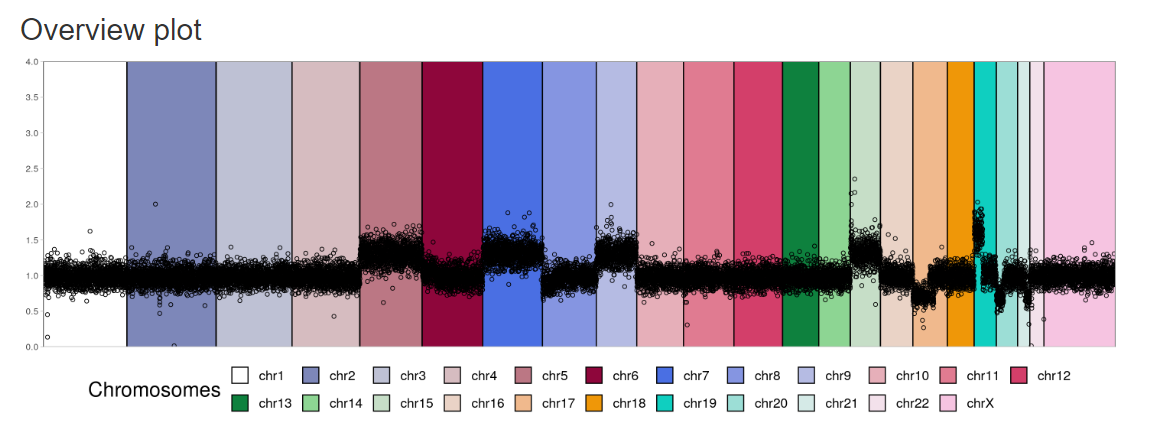
\includegraphics[width=1\textwidth]{images/cnv.png}
    \caption{Résultat de l'analyse du nombre de copies sur un échantillon de myélome multiple.}
    \label{fig:cnv}
\end{figure}

Il est alors possible de moyenner la valeur du $\log_2$ du ratio de profondeur pour les 10 sondes couvrant la région du gène \textit{TP53},  
et de l'exprimer comme une fréquence estimée de cellules délétées selon la relation suivante :

\begin{equation}
    \text{Fréquence des cellules délétées (\%)} = \left( \frac{1 - 2^{\overline{\log_2\text{Ratio}}}}{0{,}5} \right) 
    \times \frac{1}{\text{pureté}} \times 100
    \footnote{Pour exprimer le ratio de profondeur en fréquence de cellules delétées, on soustrait à 1 la valeur du ratio pour exprimer la perte relative, 
    que l'on divise par 0{,}5 qui représente la délétion monoallélique de la totatilité des cellules (une normalisation en quelque sorte). Le reste de l'expression 
    permet de corrigier par la pureté tumorale de l'échantillon, qui est le pourcentage de cellules tumorales dans l'échantillon analysé, et exprime le résultat en pourcentage.}
\end{equation}

\begin{equation}
    \text{où} \quad \overline{\log_2\text{Ratio}} = \frac{1}{n} \sum_{i=1}^{n} \log_2\text{Ratio}_i
    \footnote{Par les propriétés des logarithmes, $\overline{\log_2\text{Ratio}} = \frac{1}{n} \sum \log_2 \text{Ratio}_i = \log_2\left( \prod_{i=1}^{n} \text{Ratio}_i^{1/n} \right) = 
    \log_2\left( \sqrt[n]{\prod_{i=1}^{n} \text{Ratio}_i} \right)$, ce qui revient donc à calculer le logarithme de la moyenne géométrique.}
\end{equation}

    
Un intervalle de confiance et des statistiques de dispersion peuvent également être calculés pour évaluer la qualité de l'estimation. Cette 
approche a été implémentée dans un process \textit{Nextflow} final appelant un script Python permettant de générer au travers d'un fichier excel, 
une fréquence de délétion estimée par échantillon, et pouvant être corrigée selon la pureté tumorale (\autoref{fig:excel-tp53}). 
Par la suite l'analyse de témoins négatifs et positifs (échantillon avec ou sans délétion du gène \textit{TP53}) ont permis d'estimer 
la limite de quantification à 20 \% et de détection à 15 \% de cellules délétées.

\begin{figure}[H]
    \centering
    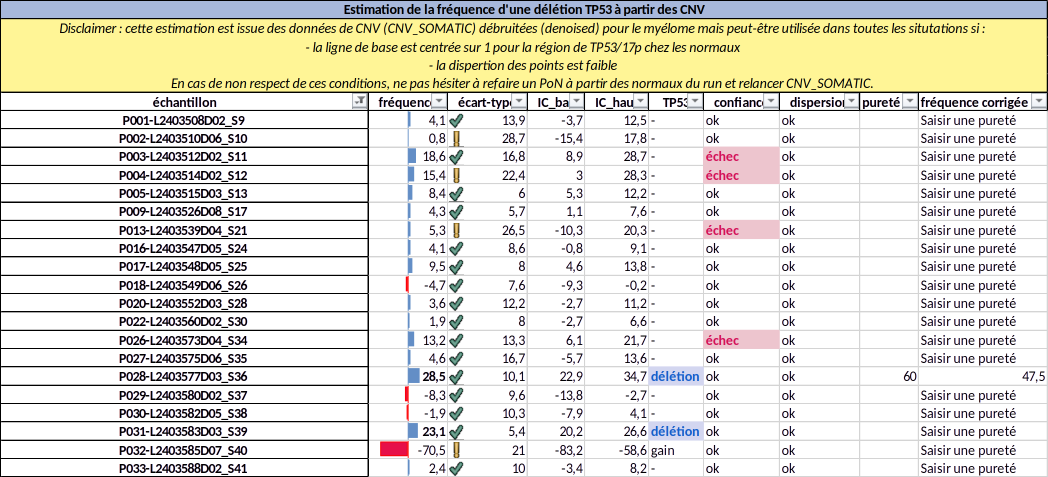
\includegraphics[width=1\textwidth]{images/excel_tp53.png}
    \caption{Résultat de l'analyse des délétions \textit{TP53} sur des échantillons de myélome multiple.}
    \label{fig:excel-tp53}
\end{figure}

\section{Seuil optimal de détection des translocations \textit{IgH}}

En lien avec la section précédente, une autre optimisation a pu être proposée concernant la recherche des translocations impliquants les \glspl{ig}.
Ces anomalies sont particulièrement importantes, considérées comme fondatrices dans l'oncogènese du \gls{mm} et leur détection se fait au \gls{chu} 
par appel de variants structuraux sur \textit{paired-end short-reads} via les \textit{caller} \textit{Manta} \cite{chenMantaRapidDetection2016a} et 
\textit{Gridss} \cite{cameronGRIDSSSensitiveSpecific2017a}. Ces deux \textit{variant-callers} fonctionnent de manière similaire en assemblant des \textit{reads} candidats
porteurs d'information structurale (\textit{split-reads}\footnote{Les \textit{split-reads} sont des lectures dont une portion s'aligne sur une région du génome 
et une autre portion sur une région distante.} et \textit{discordantly aligned reads}\footnote{Les \textit{discordantly aligned reads} 
sont des paires de lectures dont l'orientation ou la distance d'alignement est anormale par rapport à ce qui est attendu.}).

\vspace{1em}

Les résultats sont ainsi rendus sous forme de page web statique (\autoref{fig:translocation-web}), après filtrage des variants en dehors des régions d'intérêt, et en dessous d'un seuil 
de détection fixé à 10 événements supports (\textit{reads} ou paires de \textit{reads}). Des observations réalisées sur des analyses au laboratoire 
laissent à penser que certaines translocations veritables sont présentes en dessous de ce seuil fixé à 10, notamment sur des \gls{adnc}.
C'est donc concernant ce dernier, initialement fixé de manière empirique, qu'un travail d'optimisation a été entrepris afin de déterminer 
s'il permettait effectivement de discriminer de manière fiable les réarrangements pertinents des artéfacts, tout en conservant une sensibilité adéquate 
pour la détection d'événements rares. 

\begin{figure}[H]
    \centering
    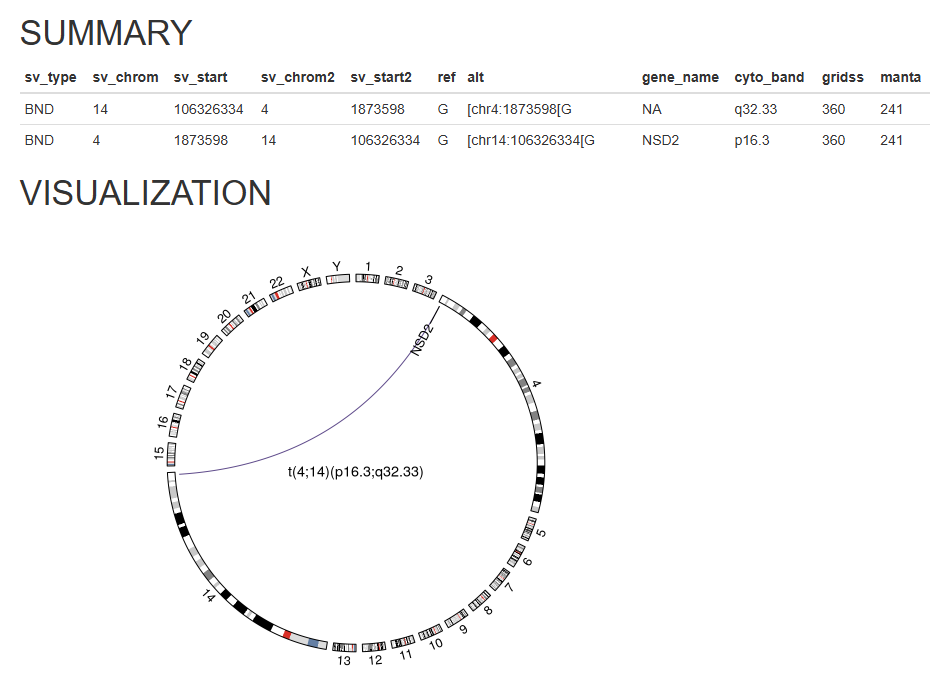
\includegraphics[width=1\textwidth]{images/translocation_web.png}
    \caption{
        Résultat de l'analyse des translocations \gls{igh} sur un échantillon de myélome multiple, 
        retrouvant ici une translocation t(4;14)(p16.3;q32.33) \textit{NSD2::IGH}.
        }
    \label{fig:translocation-web}
\end{figure}

Une manière d'aborder ce problème consiste à envisager une optimisation \textit{a posteriori}, reposant sur les nombreuses données déjà acquises, 
en formulant des hypothèses et en s'appuyant sur quelques vérités biologiques :

\begin{itemize}
    \item Les événements rapportés par \textit{Manta} et \textit{Gridss} reposent sur des signaux difficilement attribuables à des artéfacts, et peuvent donc être considérés comme fiables.
    \item Les translocations impliquant les \textit{\gls{igh}} sont des événements fondateurs, uniques et exclusifs : un patient ne présente au maximum qu'une seule translocation de ce type.
    \item À l'inverse, les translocations de type t(8;14) sont souvent secondaires, et peuvent coexister avec d'autres anomalies.
\end{itemize}

\vspace{1em}

Dans cette optique, on peut chercher à définir un seuil de détection optimisé, qui maximise le nombre de patients identifiés comme porteurs d'une translocation, 
tout en minimisant le nombre de patients présentant plusieurs anomalies, phénomène assez rare biologiquement. Ainsi on note $T$ le nombre de patients 
présentant au moins une translocation et $T_{+}$ le nombre présentant plusieurs translocations, en excluant les t(8;14). $T$ et $T_{+}$ sont alors des fonctions 
de $t$ définies sur $\mathbb{N}$ et à valeurs dans $\mathbb{N}$, $t$ désignant le seuil en dessous duquel l'anomalie n'est pas retenue. On peut donc formuler la question sous la forme d'une optimisation sous contrainte, 
où $\delta$ représente un nombre acceptable de patients présentant plusieurs translocations, et $t^*$ le seuil optimal retenu :

\begin{equation}
    t^* = \arg\max_{t} \; T(t) \quad \text{tel que} \quad T_{+}(t) \leq \delta
 \end{equation}
    
 Il est assez aisé de résoudre le problème par recherche exhaustive sur un intervalle restreint, ou graphiquement à partir des 1178 échantillons du \gls{chu} et en faisant varier 
 $t$ de $1$ à $100$ avec $\delta < 1 \%$. Ceci nous permet d'abaisser le seuil initialement à 10, à une valeur de 6 (\autoref{fig:translocation-threshold}).


\begin{figure}[H]
    \centering
    \begin{tikzpicture}
        \begin{axis}[
            width=15cm,
            height=8cm,
            xlabel={Seuil $t$},
            xmode=log,
            extra x ticks={6},
            extra x tick labels={$6$},
            ylabel={Nombre de patients},
            legend pos=north east,
            grid=major,
        ]
        \addplot[
            color=Purple,
            mark=*,
        ] table [x=t, y=T, col sep=comma] {data/threshold_analysis.csv};
        \addlegendentry{$T(t)$}

        \addplot[
            color=Goldenrod,
            mark=square*,
        ] table [x=t, y=T+, col sep=comma] {data/threshold_analysis.csv};

        \draw[dashed, thick] (axis cs:6,-100) -- (axis cs:6,1000);
        \node at (axis cs:6.5,450) [anchor=west, font=\small, text=black] {seuil $t^*$ optimal};

        \addlegendentry{$T_+(t)$}
        \end{axis}
    \end{tikzpicture}
    \caption{
        Courbes de \textcolor{Purple}{$T(t)$} et \textcolor{Goldenrod}{$T_+(t)$} à partir des 1178 échantillons du \gls{chu}.
        Le seuil optimal $t^*$ est indiqué par la ligne pointillée, il est choisi de façon à maximiser \textcolor{Purple}{$T(t)$} 
        tout en contraignant \textcolor{Goldenrod}{$T_+(t)$} en dessous de 10.
        }
    \label{fig:translocation-threshold}
\end{figure}


\section{Statistiques sur les données de \textit{Vidjil} issues du CHU de Lille}

Le dernier travail présenté dans ce rapport se situe à l'interface des deux sections précédentes. Il a consisté à réutiliser les données issues de \textit{Vidjil}, obtenues au \gls{chu}, 
afin d'établir des statistiques à grande échelle sur les résultats analysés. Deux types d'échantillons sont traités en routine : d'une part, des \glspl{lal}, pour identifier les 
réarrangements des clones tumoraux et concevoir des systèmes personnalisés de suivi de la \gls{mrd} par \gls{pcr} quantitative ; d'autre part, des \glspl{llc}, pour l'étude du taux 
d'hypermutation des gènes \textit{IGHV}. L'objectif est d'extraire et de visualiser des tendances générales à partir du volume important de données acquises.

\vspace{1em}

Le traitement des données brutes issues des analyses par \textit{Vidjil} est réalisé via un script Python (\texttt{clone.py}) qui importe les fichiers d'analyse au format \gls{json}. 
Ce script construit des objets \texttt{Vidjil} représentant chaque analyse, ainsi que des objets \texttt{Clone} extrayant les informations essentielles des clones détectés, 
telles que la taille relative, les séquences CDR3, les gènes V(D)J assignés, la productivité, etc. Une étape d'enrichissement par requête du serveur IMGT/V-QUEST 
(sans API, nécessitant donc de récupérer et traiter la page web complète) permet d'obtenir des annotations biologiques complémentaires, notamment le pourcentage d'identité des séquences V.
Par ailleurs, les métadonnées associées aux échantillons sont intégrées afin d'assurer une contextualisation clinique et biologique des résultats.

\vspace{1em}

Un second script (\texttt{process\_dir.py}) traite de manière automatisée un ensemble de fichiers d'analyse et de métadonnées situés dans un répertoire donné. 
Il agrège les informations des clones extraits selon le type d'échantillon (\gls{llc} ou \gls{lal}). Les résultats sont synthétisés dans un fichier TSV exploitable 
pour des analyses ultérieures, avec au total plus de 4000 échantillons pour 11000 clones.

\vspace{1em}

Pour finir un tableau de bord interactif a été développé à l'aide de \textit{Streamlit} (\texttt{stat\_display.py}) pour permettre l'exploration dynamique des données. 
Ce tableau de bord propose des filtres par type d'échantillon (\gls{lal}, \gls{llc} ou inconnu), par nom d'échantillon, etc. Les résultats, bien qu'intéressants, sortent du cadre 
de ce rapport ne traitant pas de la même pathologie et ne seront pas présentés ici, mais en voici une illustration pour le plaisir des yeux (\autoref{fig:vidjil-stat}) :

\begin{figure}[H]
    \centering
    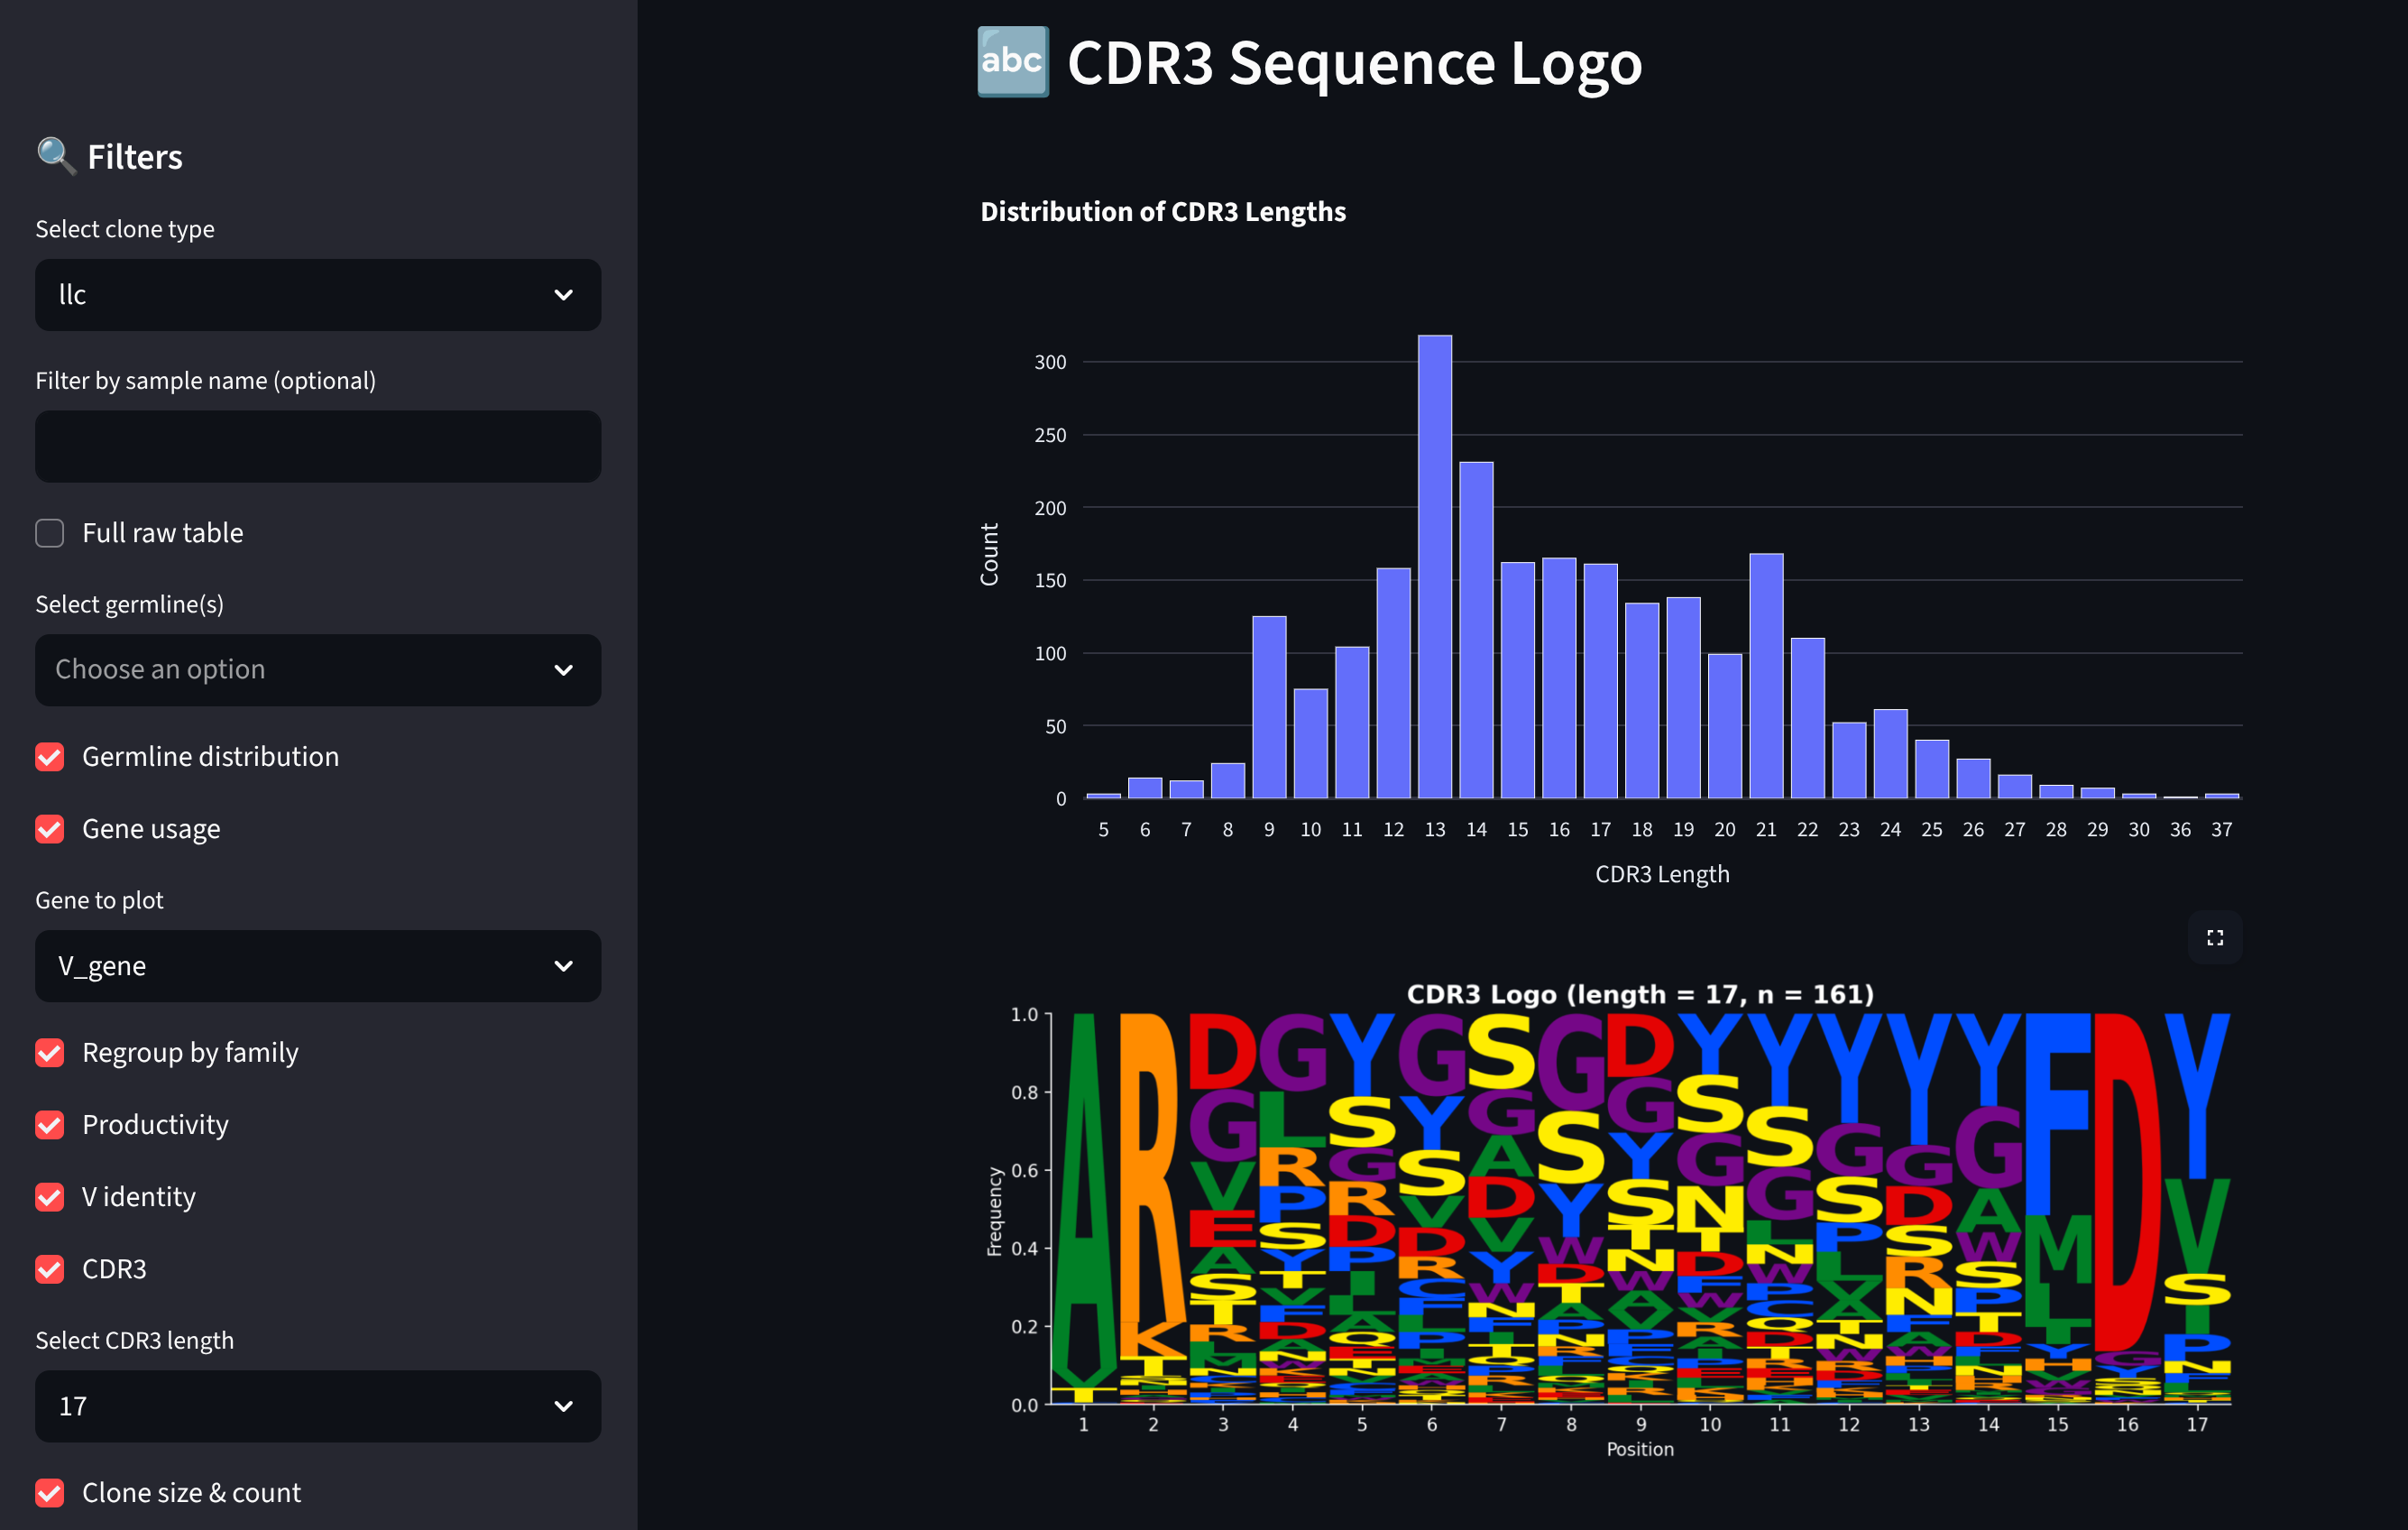
\includegraphics[width=1\textwidth]{images/vidjil_stat.png}
    \caption{
        Capture d'écran du tableau de bord pour la visualisation des statistiques des données de \textit{Vidjil}. 
        Exemple de la distribution de taille des séquences \gls{cdr}3 dans les \glspl{llc} et du logo des séquences 
        de taille 17.
        }
    \label{fig:vidjil-stat}
\end{figure}
\chapter{Discussion}
\chapter{Conclusion}

\printbibliography
\newpage

\appendix
\section*{Annexe 1 : Avis favorable du comité scientifique de la tumorothèque du CHU de Lille}

\begin{annex}[htbp]
    \begin{center}
        %\includegraphics[width=0.75\textwidth]{courrier_cstmt_mrd_mm.pdf}
        \caption{
            Avis favorable du comité scientifique de la tumorothèque du \gls{chu} pour l'étude de la \gls{mrd} dans le \gls{mm}.
            (n° d'avis CSTMT350).
        }
        \label{anx:cstmt-mrd-mm}
    \end{center}
\end{annex}

\newpage

\section*{Annexe 2 : Amorces de PCR utilisées pour l'amplification des réarrangements V(D)J en FR3}

\begin{annex}[htbp]
\centering
\tiny
\rotatebox{90}{%
\begin{tabular}{lllp{7cm}rr}
\textbf{Mix name} & \textbf{Primer ID} & \textbf{Sequence} \\
\hline

IGHcfFR3\_FP\_mix & IGHcfFR3\_VH1 & AATGATACGGCGACCACCGAGATCTACACXXXXXXXXACACTCTTTCCCTACACGACGCTCTTCCGATCTTGAGGAGCCTGAGATCTGAVGACW \\
& IGHcfFR3\_VH2 & AATGATACGGCGACCACCGAGATCTACACXXXXXXXXACACTCTTTCCCTACACGACGCTCTTCCGATCTTGACCAACATGGACMYTGTGGACA \\
& IGHcfFR3\_VH3\_a & AATGATACGGCGACCACCGAGATCTACACXXXXXXXXACACTCTTTCCCTACACGACGCTCTTCCGATCTTGAACAGYCTGAGAGCYGAGGACA \\
& IGHcfFR3\_VH3\_b & AATGATACGGCGACCACCGAGATCTACACXXXXXXXXACACTCTTTCCCTACACGACGCTCTTCCGATCTTGAACAGCCTGARARCCGAGGACA \\
& IGHcfFR3\_VH3\_c & AATGATACGGCGACCACCGAGATCTACACXXXXXXXXACACTCTTTCCCTACACGACGCTCTTCCGATCTTGAACAGHCTGAGAGCHGAGGRCA \\
& IGHcfFR3\_VH4 & AATGATACGGCGACCACCGAGATCTACACXXXXXXXXACACTCTTTCCCTACACGACGCTCTTCCGATCTTGAGCTCTGTGACYGCCGCRGACA \\
& IGHcfFR3\_VH5 & AATGATACGGCGACCACCGAGATCTACACXXXXXXXXACACTCTTTCCCTACACGACGCTCTTCCGATCTAGCAGCCTGAAGGCYTCGGACR \\
& IGHcfFR3\_VH6 & AATGATACGGCGACCACCGAGATCTACACXXXXXXXXACACTCTTTCCCTACACGACGCTCTTCCGATCTTGAACTCTGTGACTCCCGAGGACA \\
& IGHcfFR3\_VH7 & AATGATACGGCGACCACCGAGATCTACACXXXXXXXXACACTCTTTCCCTACACGACGCTCTTCCGATCTTCWGCAGCCTAAAGGCTGAGGACA \\
& IGHcfFR3\_VH & AATGATACGGCGACCACCGAGATCTACACXXXXXXXXACACTCTTTCCCTACACGACGCTCTTCCGATCTGHGGACACNGCYGTGTATTAC \\

\hline
IGHJ\_A & IGH-J-A-1 & CAAGCAGAAGACGGCATACGAGATXXXXXXXXGTGACTGGAGTTCAGACGTGTGCTCTTCCGATCTCTTACCTGAGGAGACGGTGACC \\

\hline

IGHDJ\_FP\_mix & IGHDJ\_A & AATGATACGGCGACCACCGAGATCTACACXXXXXXXXACACTCTTTCCCTACACGACGCTCTTCCGATCTGATTCYGAACAGCCCCGAGTCA \\
& IGHDJ\_B & AATGATACGGCGACCACCGAGATCTACACXXXXXXXXACACTCTTTCCCTACACGACGCTCTTCCGATCTGATTTTGTGGGGGYTCGTGTC \\
& IGHDJ\_C & AATGATACGGCGACCACCGAGATCTACACXXXXXXXXACACTCTTTCCCTACACGACGCTCTTCCGATCTGTTTGRRGTGAGGTCTGTGTCA \\
& IGHDJ\_D & AATGATACGGCGACCACCGAGATCTACACXXXXXXXXACACTCTTTCCCTACACGACGCTCTTCCGATCTGTTTRGRRTGAGGTCTGTGTCACT \\
& IGHDJ\_E & AATGATACGGCGACCACCGAGATCTACACXXXXXXXXACACTCTTTCCCTACACGACGCTCTTCCGATCTCTTTTTGTGAAGGSCCCTCCTR \\
& IGHDJ\_F & AATGATACGGCGACCACCGAGATCTACACXXXXXXXXACACTCTTTCCCTACACGACGCTCTTCCGATCTGTTATTGTCAGGSGRTGTCAGAC \\
& IGHDJ\_G & AATGATACGGCGACCACCGAGATCTACACXXXXXXXXACACTCTTTCCCTACACGACGCTCTTCCGATCTGTTATTGTCAGGGGGTGYCAGRC \\
& IGHDJ\_H & AATGATACGGCGACCACCGAGATCTACACXXXXXXXXACACTCTTTCCCTACACGACGCTCTTCCGATCTGTTTCTGAAGSTGTCTGTRTCAC \\

\hline
\end{tabular}
}
\caption{
    Séquences des amorces utilisées pour l'amplification des réarrangements V(D)J en \gls{fr}3.
    Les régions XXXXXXXX correspondent aux codes-barres spécifiques de chaque échantillons.
    }
\label{anx:primer-sequences}
\end{annex}


\end{document}
